%% Esempio per lo stile supsi
\documentclass[twoside]{supsistudent} 

\usepackage{graphicx}
\usepackage{color}

% per settare noindent
\setlength{\parindent}{0pt}

% Crea un capitolo senza numerazione che pero` appare nell'indice %
\newcommand{\problemchapter}[1]{%
  \chapter*{#1}%
  \addcontentsline{toc}{chapter}{#1}%
\markboth{#1}{#1}
}

% Numerazione delle appendici secondo norma
\addto\appendix{
\renewcommand{\thesection}{\Alph{chapter}.\arabic{section}}
\renewcommand{\thesubsection}{\thesection.\arabic{subsection}}}

\setcounter{secnumdepth}{5} 	%per avere più livelli nei titoli
\setcounter{tocdepth}{5}		%per avere più livelli nell'indice


\titolo{SaniWiki}
\studente{Antonio Daniele Mu \vspace{1em}\\Maura Clerici }
\relatore{Riccardo Mazza}
\correlatore{-}
\committente{Laura Peter - DEASS SUPSI\vspace{1em}\\Lara Barro - DEASS SUPSI}
\corso{Ingegneria informatica PAP}
\modulo{C09974 Progetto di semestre}
\anno{2018/2019}
\graphicspath{{img/}}




\begin{document}

\pagenumbering{alph}
\maketitle
\onehalfspacing
\frontmatter


\pagenumbering{roman}
\tableofcontents
\listoffigures


\newpage
\mainmatter
\pagenumbering{arabic}
\setcounter{page}{1}

\chapter{Introduzione}
Il progetto SaniWiki nasce per permettere al personale infermieristico e agli studenti di cure infermieristiche di poter accedere in maniera immediata e funzionale ad una piattaforma sempre aggiornata in cui si trovano informazioni utili alla professione e alla cura del paziente.\\

Abbiamo scelto questo progetto per il nostro lavoro di semestre essenzialmente per due ragioni, una legata al nostro percorso scolastico - lavorativo e un’altra invece legata a un lato umano, ossia al contesto in cui rientra questo progetto. Per quanto riguarda l’aspetto professionale, questo progetto ci è parso da subito interessante, perché ci offre la possibilità
di seguire interamente la progettazione di un software, partendo dalla fase di analisi iniziale fino ai suoi possibili sviluppi futuri, consentendoci inoltre di confrontarci con nuovi strumenti con i quali non abbiamo ancora familiarità.\\

Per quanto concerne invece il lato umano, questo progetto ha catturato la nostra
attenzione, perché ci permette di mettere l’informatica a servizio dell’assistenza medica,
consentendoci di facilitare il non semplice lavoro di coloro che dedicano il loro tempo ad
assistere e aiutare chi ne ha bisogno. L’idea di creare un’applicazione la cui struttura possa
essere intuitiva e efficace, così da poter fornire agli infermieri uno strumento utile per il loro
lavoro migliorando di conseguenza anche l’efficacia delle cure sui pazienti, ci è dunque
parsa interessante non solo a livello professionale, ossia per migliorare e ampliare le nostre
competenze ingegneristiche, ma anche da un punto di vista etico in quanto ci permette
di mettere l’informatica al servizio della vita.





\chapter{Analisi}

\section{Contesto}
Il progetto SaniWiki si inserisce nel contesto del Dipartimento economia aziendale, sanità e sociale della SUPSI e in particolare della formazione in cure infermieristiche. Si tratta quindi, per il momento, di un progetto interno alla SUPSI, anche se destinato a un dipartimento diverso rispetto a quello ingegneristico.

\section{Utilizzatori}
SaniWiki è rivolto agli studenti, ai docenti e agli stagisti in cure infermieristiche della SUPSI in quanto si tratta di un’applicazione che permette di accedere a un database contenente materiale didattico costantemente aggiornato relativo al mondo delle cure infermieristiche. Il progetto non è però rivolto esclusivamente agli studenti, e non ha dunque una finalità esclusivamente didattica, in quanto potrà essere utilizzato, in futuro, anche dal personale infermieristico che opera in Ticino. Gli utilizzatori, dapprima docenti e studenti, potranno quindi potenzialmente espandersi, in un secondo tempo, a tutto il personale infermieristico.

\section{Pre-condizioni}
Un prototipo dell’applicazione web SaniWiki esisteva già prima che ci mettessimo a lavorare a questo progetto, in quanto era stato realizzato l’anno scorso dal dipartimento della SUPSI DEASS. Non si è dunque trattato di creare un’applicazione ex novo, ma si è trattato di elaborare una riflessione sull’ applicazione già esistente e soprattutto sugli aspetti che in essa dovevano essere modificati, adattati, resi più efficaci e incisivi. Si tratta quindi di un lavoro di progettazione molto diverso da quello che si potrebbe fare progettando un’applicazione da zero. Occorre infatti valutare i diversi elementi già presenti e chiedersi costantemente se sono funzionali allo scopo per cui sono stati creati, se potrebbero esserlo maggiormente, se il modo di accedervi è lineare e intuitivo per l’utilizzatore, se la grafica è più o meno convincente. Si tratta dunque di semplificare, limare, rendere l’esperienza dell’utilizzatore più facile e intuitiva, tenendo conto del lavoro che è stato fatto da chi originariamente ha concepito l’applicazione e dell’idea iniziale che li ha portati a progettarla in un certo modo, così da sfruttarne i punti forti, non vanificando il lavoro di chi ci ha preceduto, ed eliminare invece gli aspetti meno funzionali.

\section{Requisiti}

\subsection{Contenuti}
Il principale requisito a livello contenutistico è quello di avere a disposizione uno schedario virtuale, in cui poter inserire le nozioni infermieristiche necessarie allo svolgimento della professione e all’apprendimento degli studenti. Relativamente a questo requisito si rivela necessario creare delle categorie e delle sezioni in cui poter organizzare la massa di informazioni utili per tema e per argomento. L’organizzazione dei contenuti in sezioni, categorie e argomenti dovrebbe far sì che sia ricercare le informazioni sia inserirle diventi più semplice per l’utente in quanto esse sono raggruppate secondo un criterio logico e coerente.\\
Un altro requisito legato al contenuto è quello di poter caricare facilmente nella piattaforma non solo testi, ma anche documenti audiovisivi e multimediali come immagini, grafici, tabelle o video.

\subsection{Grafici}
A livello grafico il requisito principale è un aspetto pulito, intuitivo e di facile interpretazione anche a livello puramente visivo. Si tratta dunque di creare icone che rimandino per analogia ai concetti e ai contenuti presenti nelle diverse categorie e rispettivamente sezioni. Siccome la SUPSI possiede una sua identità grafica, ci è stato richiesto di adattare la nostra piattaforma alle sue disposizioni relative a fonts, colori e layout web.

\subsection{Usabilità}
Per quanto riguarda i requisiti legati agli aspetti sistemistici, il più importante è sicuramente l’utilizzo all’applicazione tramite tablet. Allo stesso tempo, i docenti devono poter inserire il contenuto in modo agevole; per questo motivo è necessario rendere accessibile l'applicazione anche tramite browser.\\\\

\section{Obiettivi}
Gli obiettivi, nel dettaglio e in sintesi di quest'applicazione web, sono i seguenti:
\begin{itemize}
\item Sviluppare un prodotto utilizzabile tramite tablet
\item Creare un’interfaccia che preveda un utilizzo semplice e intuitivo
\item Racchiudere in un database tutte le conoscenze utili alla professione
\item Creare degli strumenti in cui sia possibile caricare facilmente i contenuti testuali e multimediali
\item Creare una grafica funzionale e coerente con il progetto
\end{itemize}





\chapter{Studio delle Soluzioni}

\section{Situazione attuale}
Per realizzare il progetto ci siamo basati, come detto, su un primo prototipo di SaniWiki precedentemente realizzato da un altro informatico della SUPSI. Questo prototipo, che non è mai stato lanciato, è un CMS che prevede un portale con un database in stile Wikipedia. Il motivo principale per cui questo CMS non è mai stato lanciato risiede nel fatto che non è adattato a tablet e dispositivi mobili; inoltre non appare particolarmente intuitivo e le committenti hanno riscontrato difficoltà nell’inserire nuovi testi e schede contenutistiche al suo interno così come nel trovare rapidamente le informazioni utili. Graficamente non soddisfa poi i gusti e le necessità delle committenti che desiderano uno strumento più semplice e facile da utilizzare. 
Nel concepire il nostro progetto siamo dunque partiti da questa prima versione di SaniWiki, di cui abbiamo analizzato i contenuti e gli aspetti grafici e ingegneristici, per poi passare alla progettazione delle categorie, delle sezioni e degli altri aspetti di cui parleremo in dettaglio nel capitolo dedicato all'implementazione.

\subsection{Vecchia piattaforma}
La vecchia piattaforma già presente è stata creata grazie al supporto di un Content Management System di terze parti (Tiki Wiki). Nella pagina principale è possibile accedere alla ricerca di contenuti e alle pagine che contengono le informazioni messe a disposizione (Figura 3.1).\\
\begin{figure}[!h]
\centering
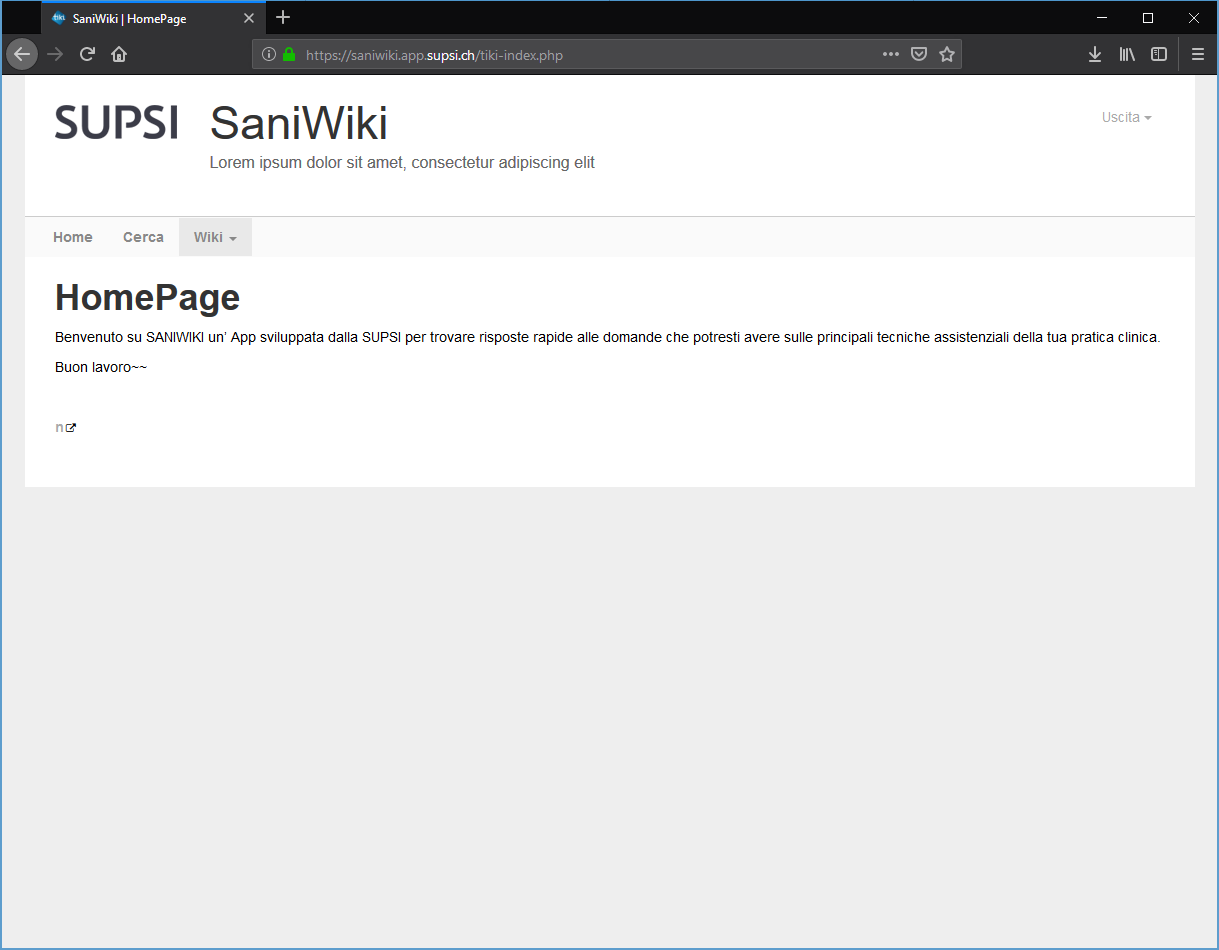
\includegraphics[scale=0.25]{saniold_home.png}
\caption{Vecchia piattaforma - Home page}
\end{figure}

Le pagine create sono raccolte in una tabella che permette di sapere quando è stata apportata l'ultima modifica e da chi (Figura 3.2).\\
\begin{figure}[!h]
\centering
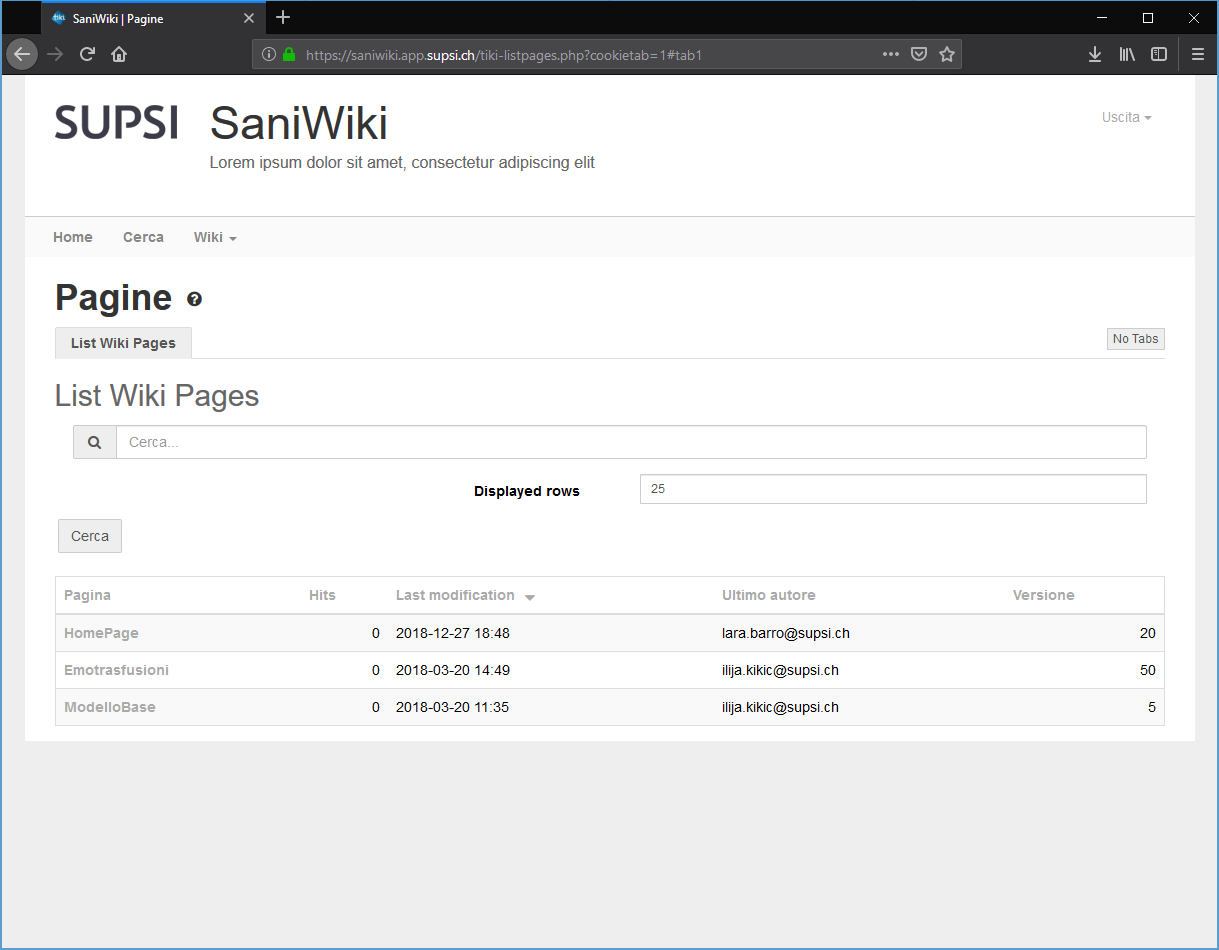
\includegraphics[scale=0.25]{saniold_list.png}
\caption{Vecchia piattaforma - Visualizzazione di tutte le pagine presenti}
\end{figure}

Accedendo a una pagina completa, vengono visualizzate delle sezioni con le rispettive icone, identiche per tutte le altre pagine: "Introduzione", "Preparazione al paziente", "Materiale", "Procedura", "Red flags", "Complicanze", ecc... (Figura 3.3)\\\\\\\\\\\\
\begin{figure}[!h]
\centering
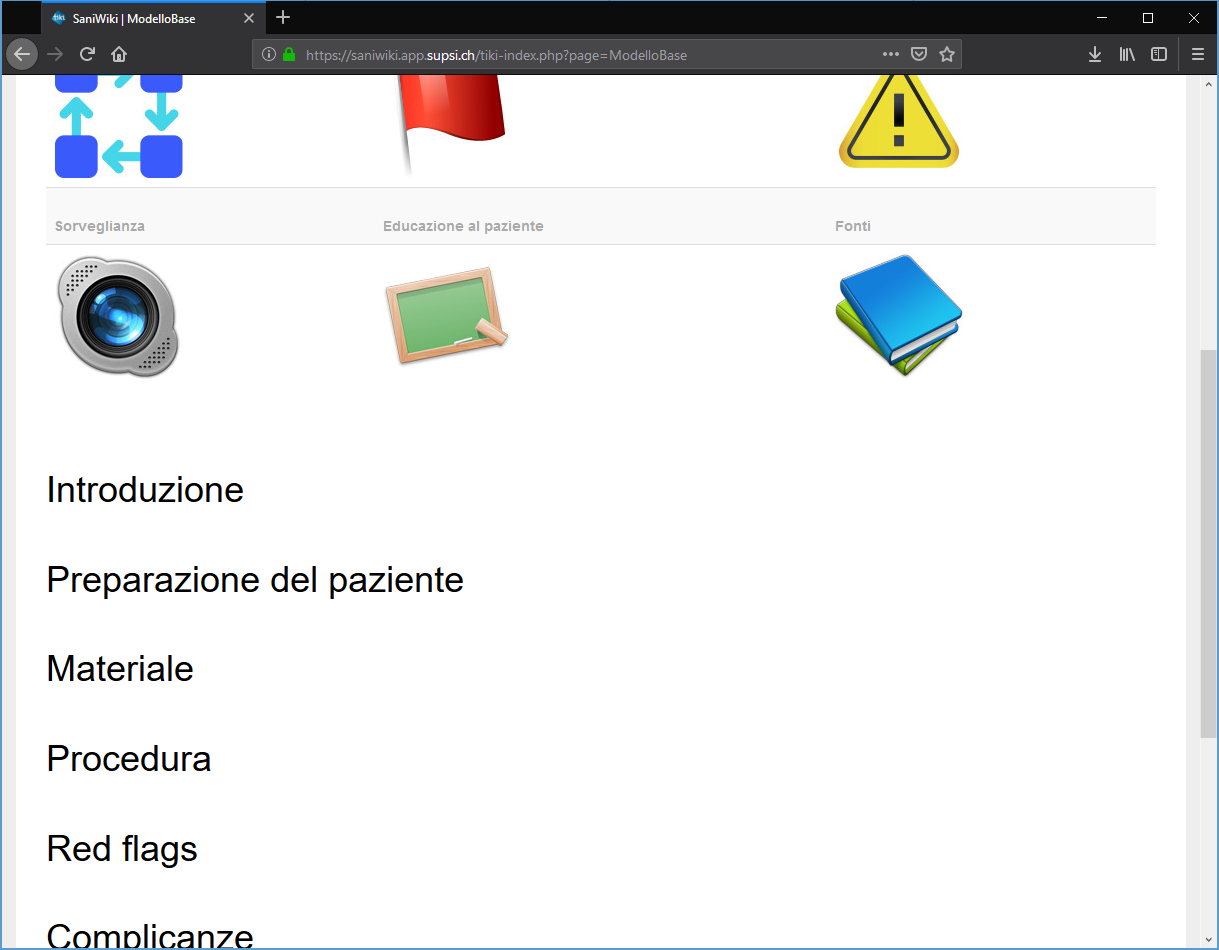
\includegraphics[scale=0.23]{saniold_template.png}
\caption{Vecchia piattaforma - Pagina modello per l'inserimento dei contenuti}
\end{figure}
\\\\\\

\section{Use cases}
Di seguito sono presentati tre diagrammi di casi d'uso: Management System (Figura 3.4), Handle Category (Figura 3.5) e User Management (Figura 3.6).\\\\\\\\\\\\\\\\\\\\\\\\\\\\\\\\
\begin{figure}[!h]
\centering
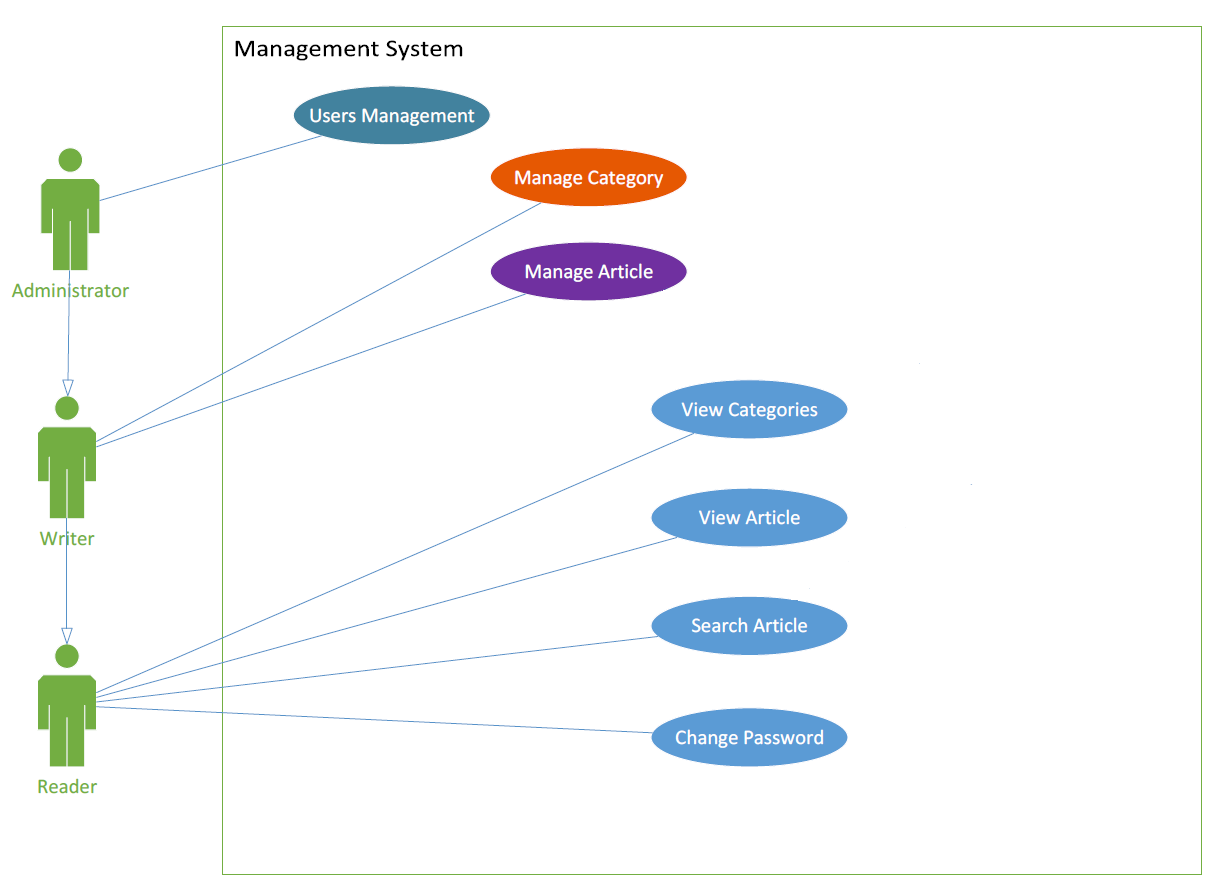
\includegraphics[scale=0.3]{usecase_management.png}
\caption{Use Case - Management System}
\end{figure}
\begin{figure}[!h]
\centering
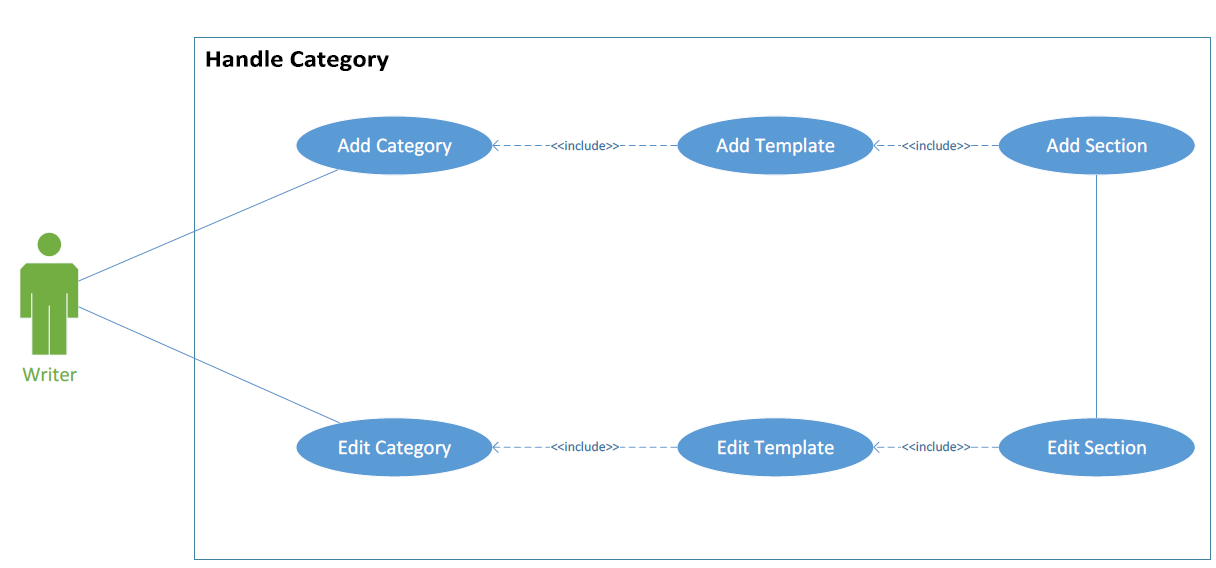
\includegraphics[scale=0.3]{usecase_writer.png}
\caption{Use Case - Handle Category}
\end{figure}
\begin{figure}[!h]
\centering
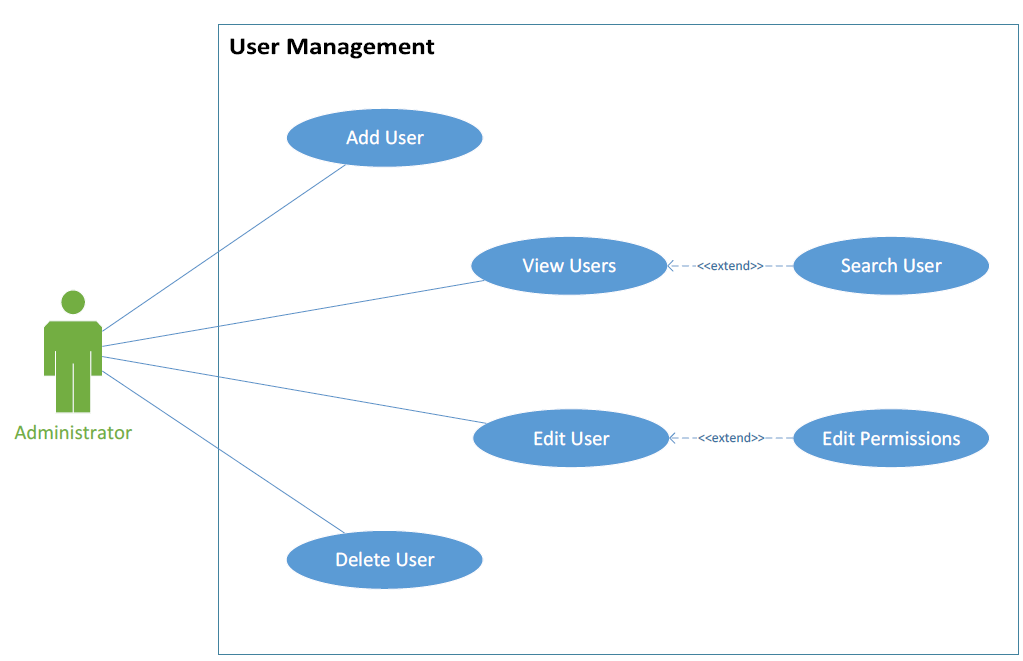
\includegraphics[scale=0.3]{usecase_administrator.png}
\caption{Use Case - User Management}
\end{figure}

\section{Scelte effettuate}
Inizialmente avevamo pensato di realizzare un’applicazione adatta esclusivamente a dispositivi mobili, considerando la possibilità di utilizzare il framework Ionic, il quale permette di sviluppare applicazioni web native per dispositivi mobili Android e iOS. Dopo aver riflettuto a lungo su questa possibilità, ci siamo però resi conto che l’utilizzo dell’applicazione unicamente tramite dispositivi mobili avrebbe comportato alcuni limiti non indifferenti rispetto agli scopi del progetto; in particolare sarebbe stato scomodo l'inserimento di contenuti tramite tablet, opzione scomoda per chi deve inserire nel database testi di una certa lunghezza. Scrivere su un PC attraverso una tastiera è certamente più comodo che scrivere direttamente su un tablet e, considerato anche il fatto che probabilmente molti docenti redigono i loro testi su un computer e quindi la maggior parte dei loro documenti è salvata in esso, abbiamo infine deciso di propendere verso una scelta maggiormente mirata ai bisogni degli utilizzatori e dei destinatari del nostro progetto. La scelta finale è stata dunque quella di creare un’applicazione web in modo che SaniWiki fosse accessibile da fonti diverse, quindi sia attraverso un tablet sia attraverso un PC. Applicazione che può successivamente espandersi, tramite api, per implementare Web App native.
Il linguaggio di programmazione PHP è stato invece scelto perché rende più accessibile la manutenzione del relativo web server rispetto a un linguaggio come Java.\\
Per quanto riguarda i Framework, ne abbiamo testati due, ossia Lumen, un microframework di Laravel che non predispone di un template engine e sarebbe stato facilmente integrabile con Ionic, e Laravel. Avendo però Lumen meno funzionalità di Laravel, dato che appunto non utilizza Blade come template engine, alla fine abbiamo scelto di scartare Lumen e utilizzare Laravel per lo sviluppo dell'applicazione web, poiché quest'ultimo offre molti strumenti sia per quanto concerne lo sviluppo sia per quanto concerne le parti grafiche; inoltre esso semplifica e rende più dinamico il lavoro del programmatore.

\section{Ambiente di sviluppo}

\subsection{Framework e librerie}
Il Framework utilizzato è Laravel 5.7, ossia l’ultima versione disponibile. Abbiamo scelto di utilizzare l’ultima versione, perché le committenti erano preoccupate della possibile manutenzione e degli aggiornamenti del software e questa scelta consente invece di non rendere necessaria, almeno per i primi due anni dalla sua installazione, la manutenzione o l’aggiornamento dell’applicazione.\\
Laravel utilizza diverse librerie tra cui Bootstrap 4, libreria che permette di adattare i contenuti grafici ai tablet e ai dispositivi mobili, e SCSS per quanto riguarda invece la parte grafica.

\subsection{Database Management System}
Il sistema scelto per gestire il database è MySQL perché si interfaccia bene con il linguaggio PHP e, dato che il nostro database è relativamente piccolo, poco complesso e con poche tabelle, non necessita di ottimizzazioni particolari o altre estensioni specifiche per farlo funzionare in maniera ottimale.

\subsection{Database Schema}
\begin{figure}[!h]
\centering
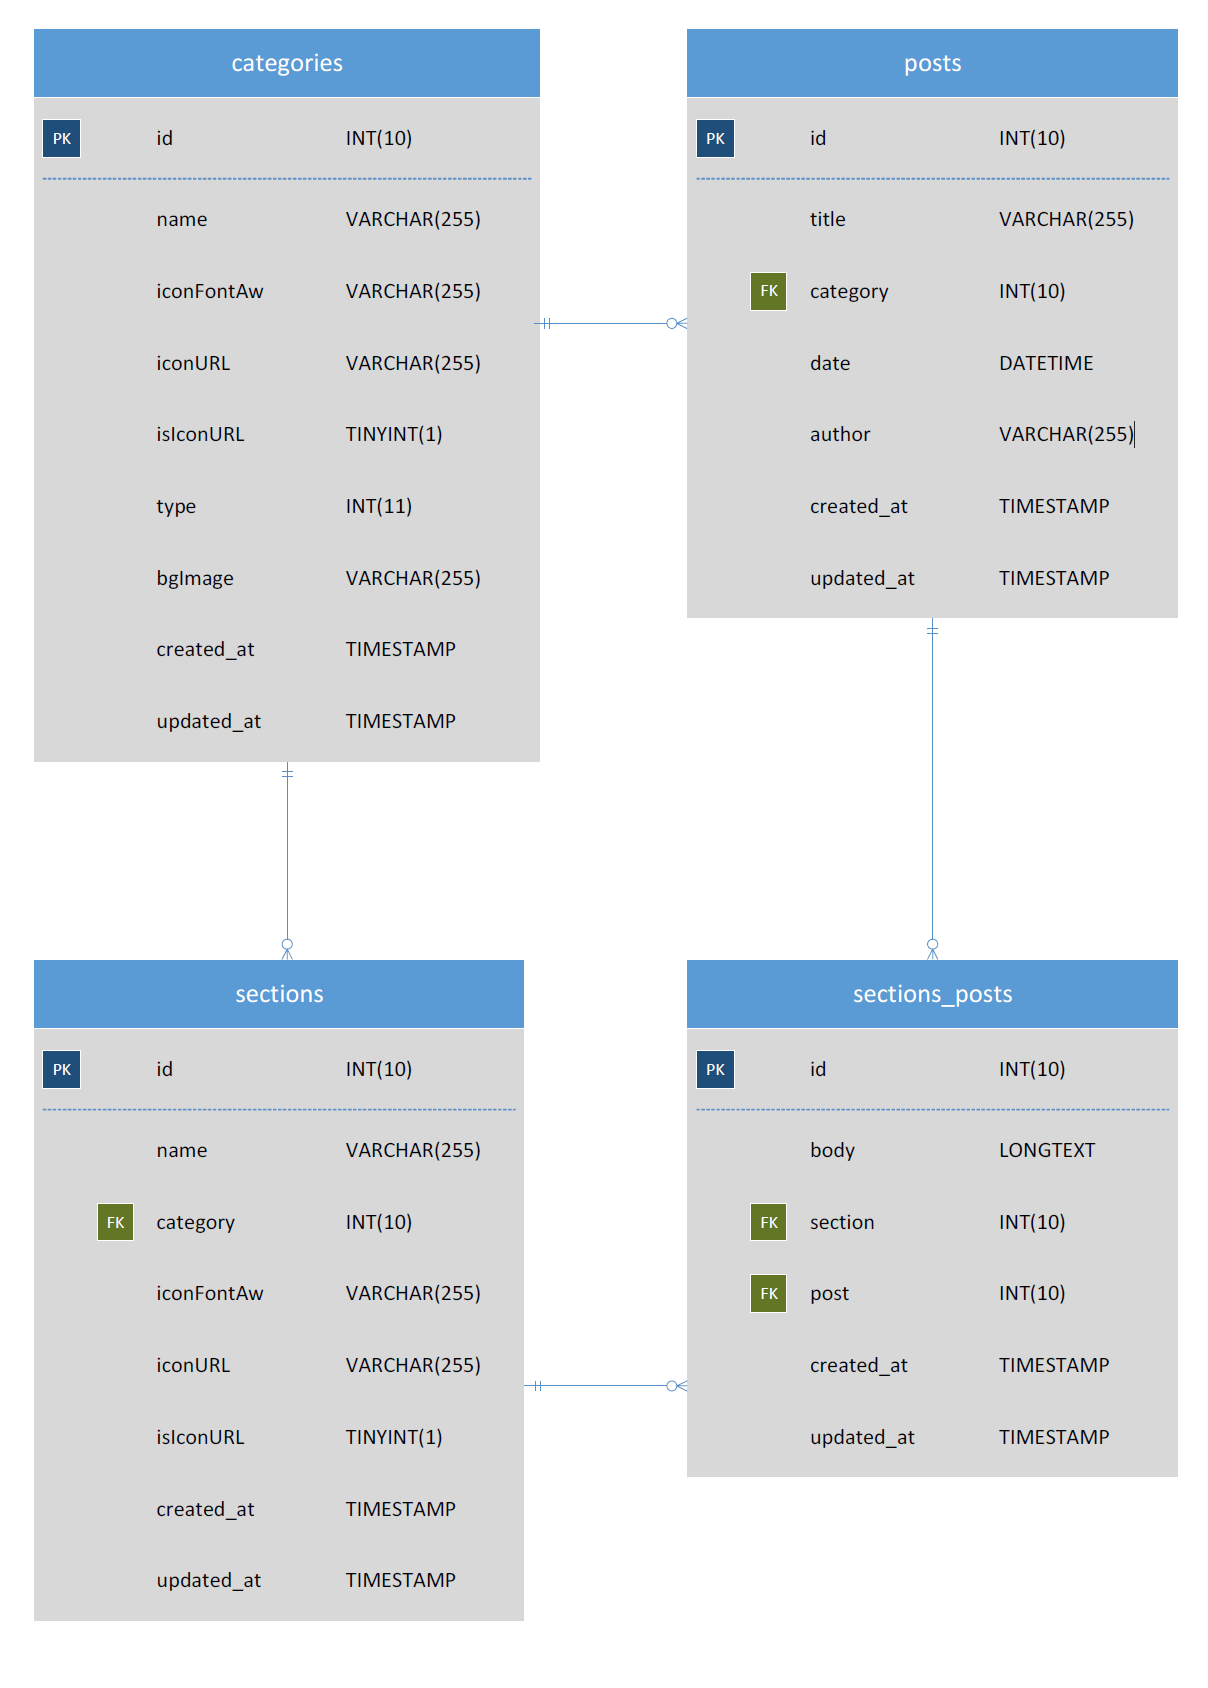
\includegraphics[scale=0.6]{schema_1.PNG}
\caption{Schema del database implementato - 1}
\end{figure}
\begin{figure}[!h]
\centering
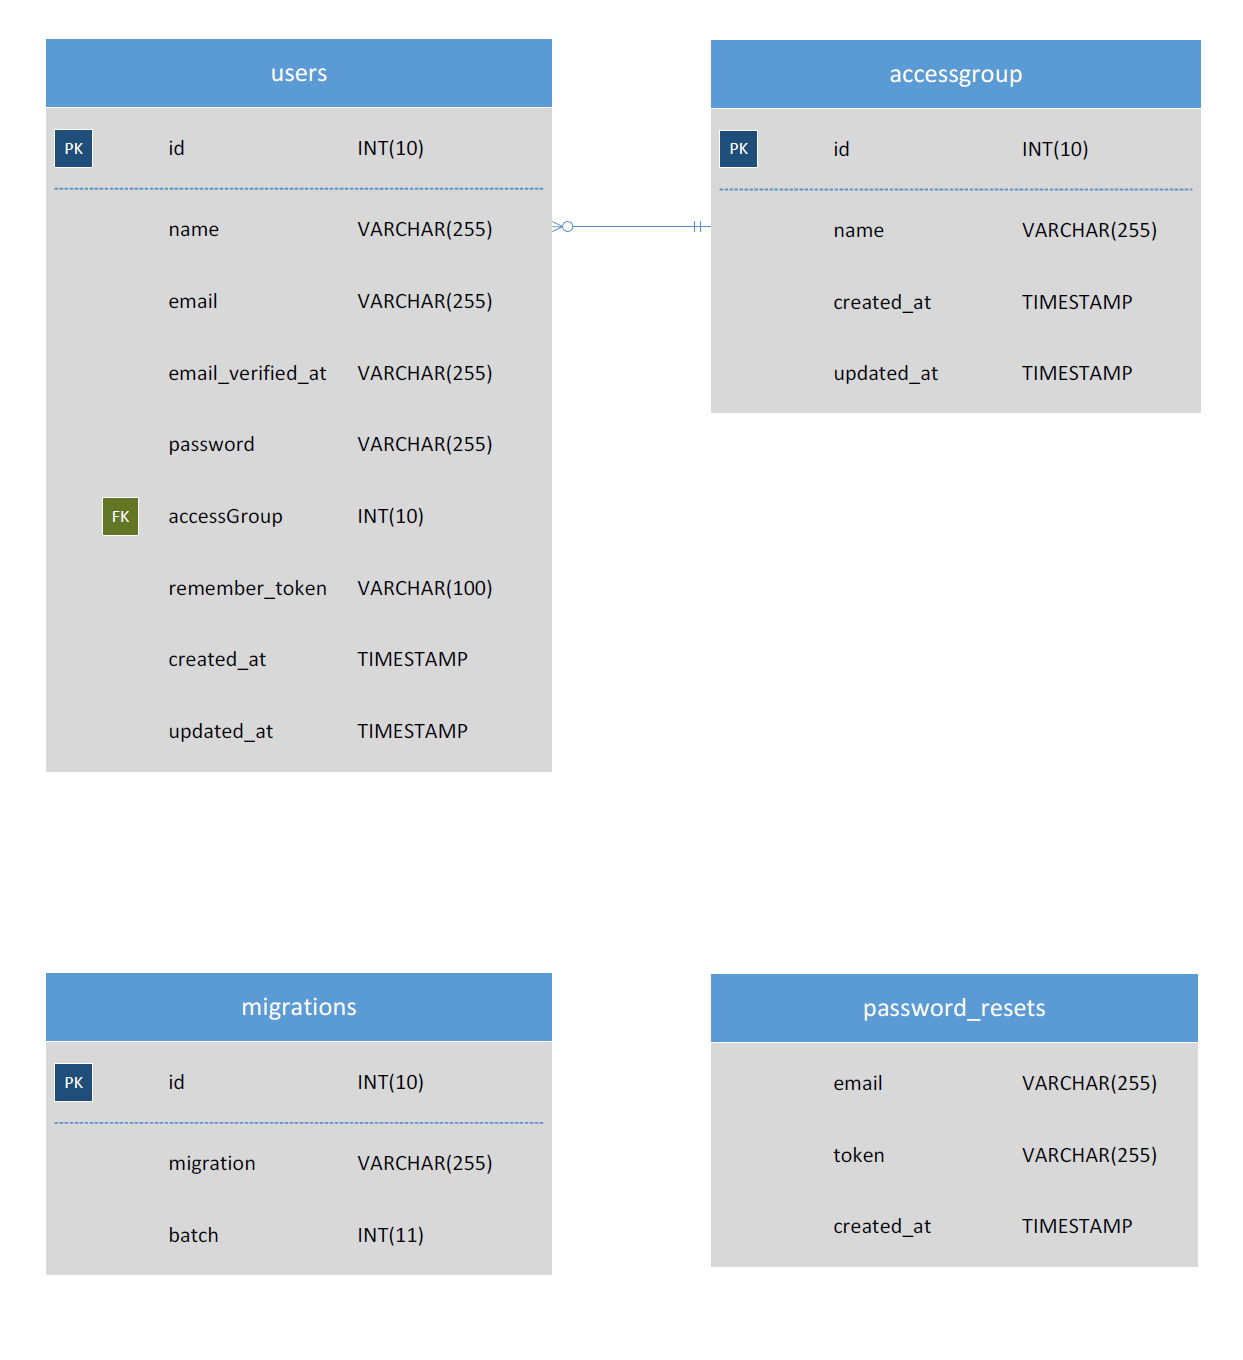
\includegraphics[scale=0.6]{schema_2.PNG}
\caption{Schema del database implementato - 2}
\end{figure}

\subsection{Web Server}
Per quanto riguarda il server su cui ospitare l'applicazione abbiamo chiesto alla scuola di metterci a disposizione un server Linux. Visto che abbiamo scelto di utilizzare un linguaggio PHP e come DBMS abbiamo scelto MySQL, abbiamo ritenuto che la scelta più pertinente fosse quella di utilizzare un server Linux con installato Apache. Questo server, che ospita la nostra piattaforma, ci ha permesso di testare la funzionalità della nostra applicazione e di renderla accessibile all’intera rete SUPSI.

\section{Strumenti utilizzati}
Abbiamo utilizzato PHP Storm, programma della Jet Brain, come IDE, per sviluppare SaniWiki e installare il Framework Laravel da zero. Tramite le linee di comando di Laravel abbiamo poi potuto costruire gli altri elementi necessari per realizzare il nostro progetto. 





\chapter{Implementazione}

\section{Login e Sicurezza}
È stato implementato un sistema di login che permette l'accesso ad utenti già creati da un amministratore. I visitatori non hanno la possibilità di registrarsi, come da richiesta dei committenti. Quando un visitatore tenta di accedere ad una pagina interna viene rediretto automaticamente alla pagina di Login (Figura 4.1).
\begin{figure}[!h]
\centering
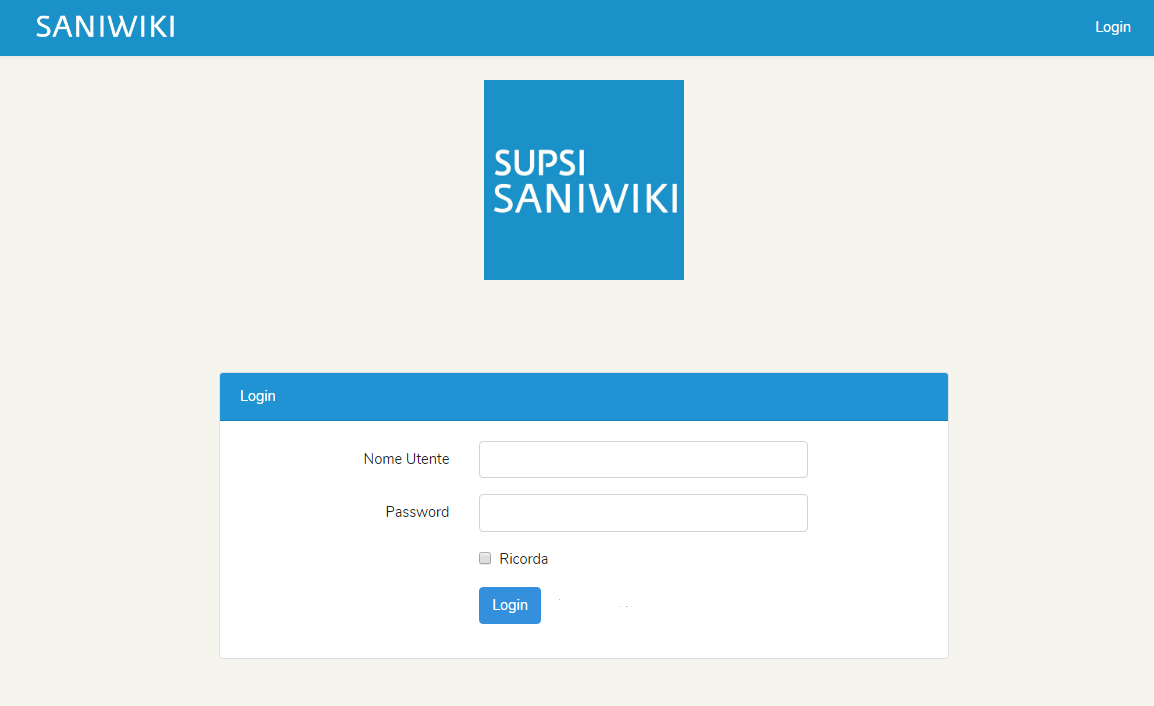
\includegraphics[scale=0.4]{saniwiki_login.png}
\caption{Pagina di Login}
\end{figure}
\\ \\ \\
Esistono tre livelli di accesso diversi per utilizzare la piattaforma:\\
\begin{itemize}
\item Amministratore: può leggere tutti i contenuti, come aggiungere, modificare ed eliminare categorie, sezioni, articoli e testi. Inoltre può aggiungere, modificare ed eliminare gli utenti.\\
\item Lettura/Scrittura: può leggere tutti i contenuti, come aggiungere, modificare ed eliminare categorie, sezioni, articoli e testi.\\
\item Lettura: può unicamente leggere tutti i contenuti.\\
\end{itemize}

\section{Gestione Utenti}
La pagina di gestione degli utenti è raggiungibile cliccando sul menu in alto a destra "Gestione Utenti", visibile unicamente dagli amministratori (Figura 4.2).
\begin{figure}[!h]
\centering
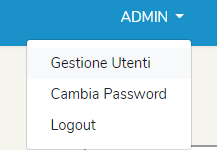
\includegraphics[scale=0.6]{saniwiki_linkgestioneutenti.png}
\caption{Menu per la Gestione Utenti}
\end{figure}
\\\\
L'interfaccia mostra una tabella che raccoglie tutti gli utenti salvati nel database, con i rispettivi ID, nomi, e-mails e livelli di accesso (Figura 4.3).\\
\begin{figure}[!h]
\centering
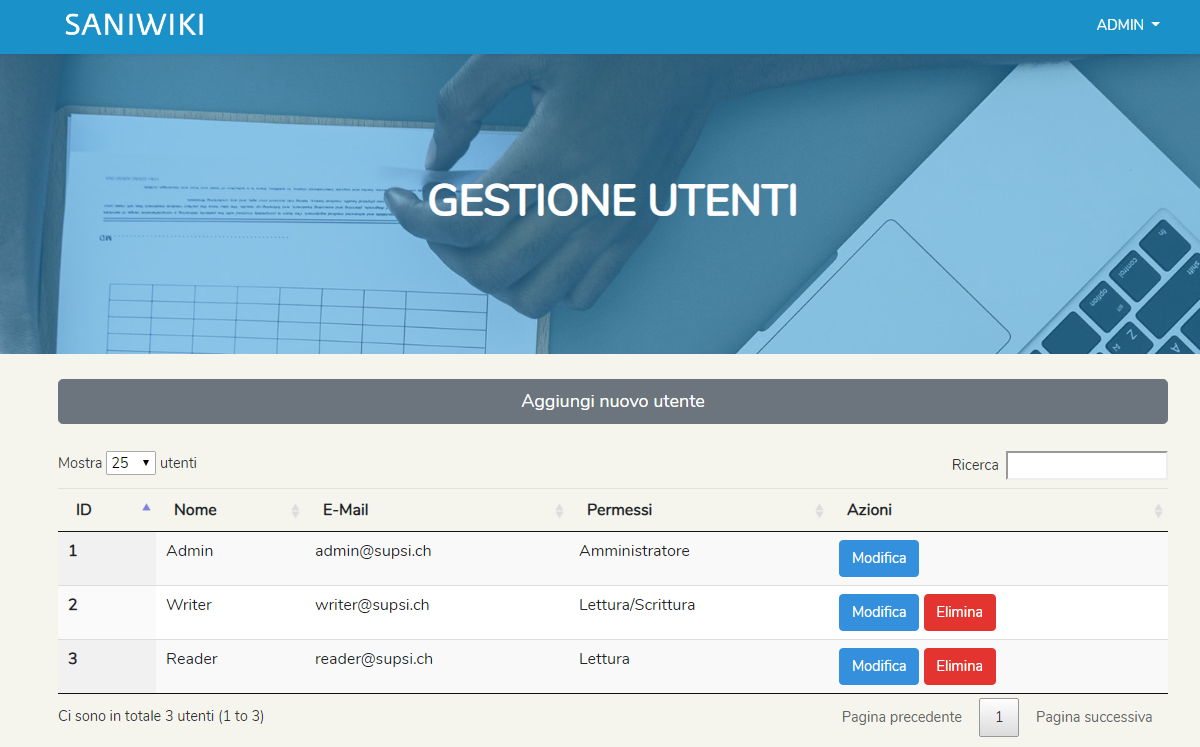
\includegraphics[scale=0.4]{saniwiki_gestioneutenti.png}
\caption{Tabella di Gestione Utenti}
\end{figure}
\\
Tramite la ricerca rapida a destra è possibile filtrare i contenuti digitando parti di ID, nomi, e-mails e gruppi di accesso istantaneamente. Esiste una pagination con la quale è possibile visualizzare un numero definito di utenti (25 di default) sulla stessa pagina. Per ogni utente sono visibili i pulsanti di modifica ed eliminazione nella colonna "Azioni" della tabella.\\
Nella modifica di un utente è possibile modificare i campi relativi al nome, indirizzo e-mail, password e livello di accesso (permessi). Per quanto riguarda la password, essa viene codificata utilizzando l'algoritmo di crittografia SHA1 prima di essere salvata nel database (Figura 4.4).\\\\
\begin{figure}[!h]
\centering
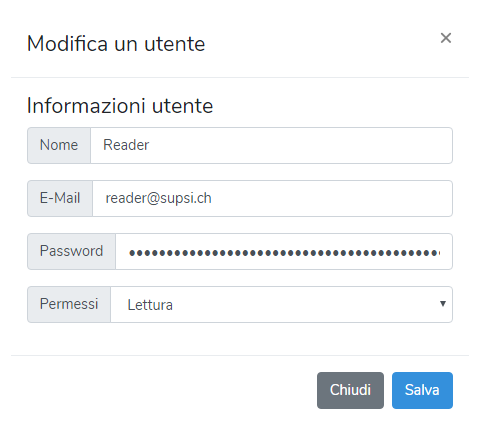
\includegraphics[scale=0.6]{saniwiki_modificautente.png}
\caption{Modifica Utente}
\end{figure}
Prima di eliminare un utente, viene sempre richiesta la conferma per eseguire l'azione (Figura 4.5).
\begin{figure}[!h]
\centering

\includegraphics[scale=0.6]{saniwiki_eliminautente.png}
\caption{Eliminazione Utente}
\end{figure}

\section{Cambio password}
Tutti gli utenti hanno la possibilità, tramite il menu in alto a destra "Cambia Password", di modificare la propria password.
Il sistema rende possibile la modifica solo se il testo immesso nei due campi "Password" e "Ripeti password" coincide.
La password viene codificata con l'algoritmo di crittografia SHA1 e salvata nel database (Figura 4.6).\\
\begin{figure}[!h]
\centering
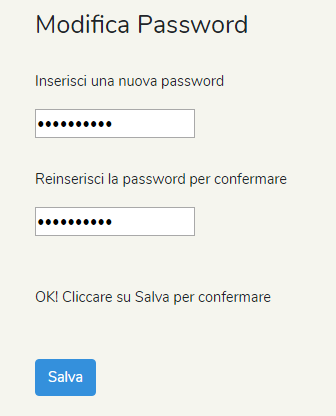
\includegraphics[scale=0.6]{saniwiki_modificapassword.png}
\caption{Modifica della password}
\end{figure}

\section{Categorie}
La pagina principale a cui si viene rediretti dopo aver eseguito l'accesso, mostra tutte le categorie presenti (Figura 4.7).\\
\begin{figure}[!h]
\centering
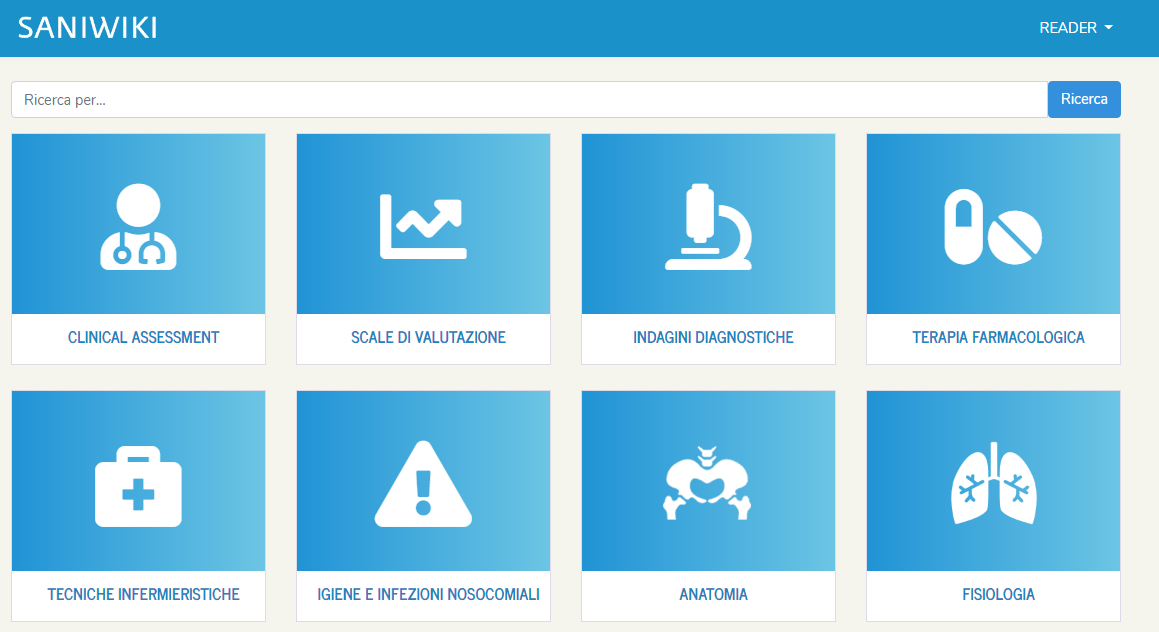
\includegraphics[scale=0.4]{saniwiki_categorie.png}
\caption{Pagina Principale - Lista Categorie}
\end{figure}
\\\\
In ogni categoria vengono definite una o più sezioni, grazie alle quali sarà possibile creare una sorta di template per strutturare gli articoli che faranno parte di una determinata categoria.\\
Gli utenti aventi il permesso di scrittura, visualizzano i pulsanti di modifica ed eliminazione per ogni categoria (Figura 4.8).
\begin{figure}[!h]
\centering

\includegraphics[scale=0.6]{saniwiki_modificaeliminacategoria.png}
\caption{Categoria - Permessi di Scrittura}
\end{figure}
Inoltre, gli stessi utenti visualizzano un riquadro ulteriore che permette l'aggiunta di nuove categorie (Figura 4.9).\\ \\ \\ \\ \\ \\
\begin{figure}[!h]
\centering

\includegraphics[scale=0.6]{saniwiki_aggiungicategorie.png}
\caption{Icona per l'aggiunta di una Categoria}
\end{figure}
\\\\
Nell'aggiunta di una nuova categoria, viene richiesto il nome, un ordine di visualizzazione e la relativa icona. Cliccando su "Avanti" dopo aver inserito le prime informazioni, è possibile definire tutte le sezioni per la categoria (Figura 4.10).\\
\begin{figure}[!h]
\centering
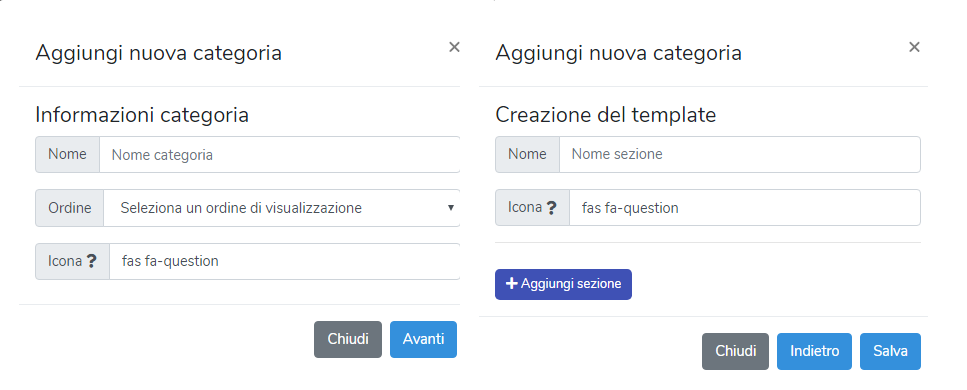
\includegraphics[scale=0.5]{saniwiki_aggiuntacategoria.png}
\caption{Aggiunta di una nuova Categoria}
\end{figure}
\\\\
Nella modifica di una categoria, vengono riportate tutte le informazioni relative alla categoria che si sta modificando, con tutte le sue sezioni. Non è possibile eliminare o aggiungere ulteriori sezioni nella modifica di una categoria (Figura 4.11).
\begin{figure}[!h]
\centering
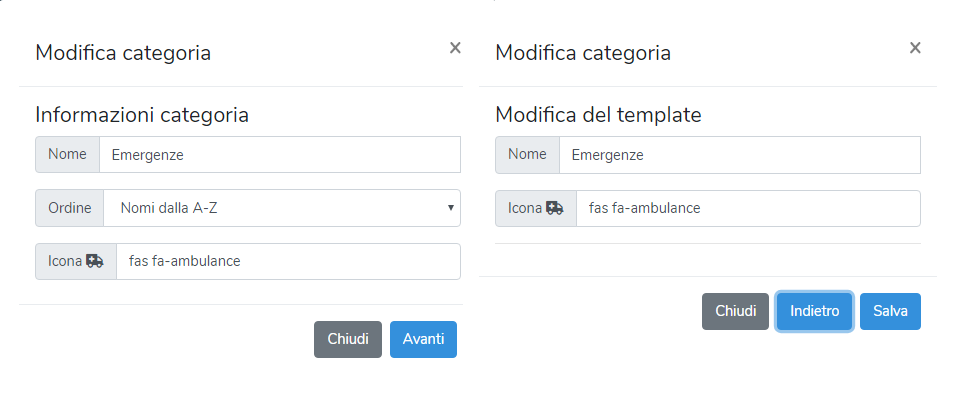
\includegraphics[scale=0.5]{saniwiki_modificacategoria.png}
\caption{Modifica di una Categoria}
\end{figure}
\\
Per eliminare una categoria, occorre confermare, in quanto vengono eliminate anche le relative sezioni e articoli appartenenti a quella categoria (Figura 4.12).\\\\\\\\\\\\\\\\
\begin{figure}[!h]
\centering
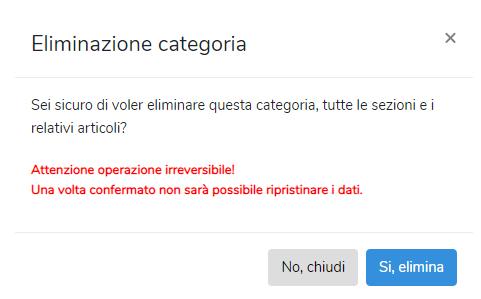
\includegraphics[scale=0.6]{saniwiki_eliminacategoria.png}
\caption{Eliminazione di una Categoria}
\end{figure}

\section{Ordine di visualizzazione}
Sono stati definiti, con i committenti, i seguenti ordine di visualizzazione degli articoli contenuti nelle categorie:\\
\begin{itemize}
\item Nomi dalla A-Z: tutti gli articoli vengono mostrati in ordine alfabetico dalla A alla Z.\\
\item Dal più recente: tutti gli articoli, a partire dall'ultimo creato al primo.\\
\item Dal più vecchio: tutti gli articoli, a partire dal più vecchio al più recente.\\
\end{itemize}

\section{Sezioni}
Le sezioni vengono definite in una categoria e strutturano tutti gli articoli contenuti nella stessa. Infatti, in tutti gli articoli appartenenti ad una categoria sono presenti sempre le stesse sezioni; questo impone il mantenimento di una struttura ed un ordine nella presentazione degli articoli (Figura 4.13).\\\\\\\\\\
\begin{figure}[!h]
\centering

\includegraphics[scale=0.4]{saniwiki_sezioni.png}
\caption{Sezioni in un Articolo}
\end{figure}

\section{Articoli}
Gli articoli possono appartenere ad una sola categoria e, nella pagina principale, quando l'utente clicca su ognuna di esse, vengono presentati tutti gli articoli collegati ad una determinata categoria in forma di tabella. (Figura 4.14)\\
\begin{figure}[!h]
\centering
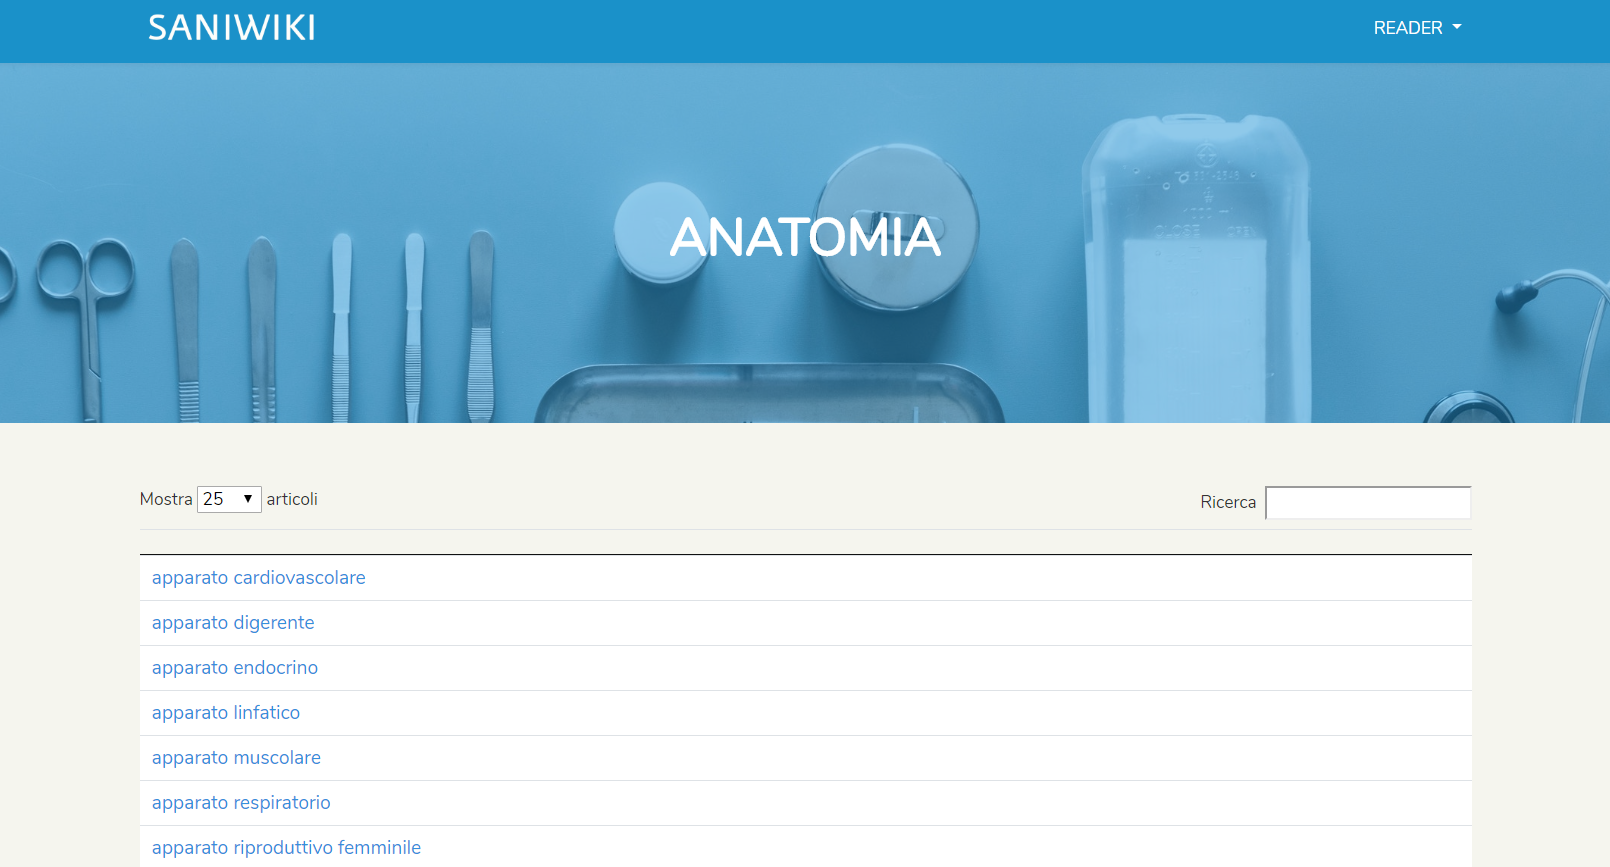
\includegraphics[scale=0.4]{saniwiki_articoli.png}
\caption{Lista di Articoli}
\end{figure}
\\
Gli utenti con permessi di scrittura hanno la possibilità di aggiungere, modificare ed eliminare ogni articolo. L'aggiunta dello stesso si presenta richiedendo unicamente un titolo e, dopo aver cliccato su "Salva", l'utente viene reindirizzato ad un'altra pagina in cui ha la possibilità, tramite un editor di testo WYSYWYG, di scrivere il contenuto sotto ad ogni sezione. (Figura 4.15)\\
\begin{figure}[!h]
\centering
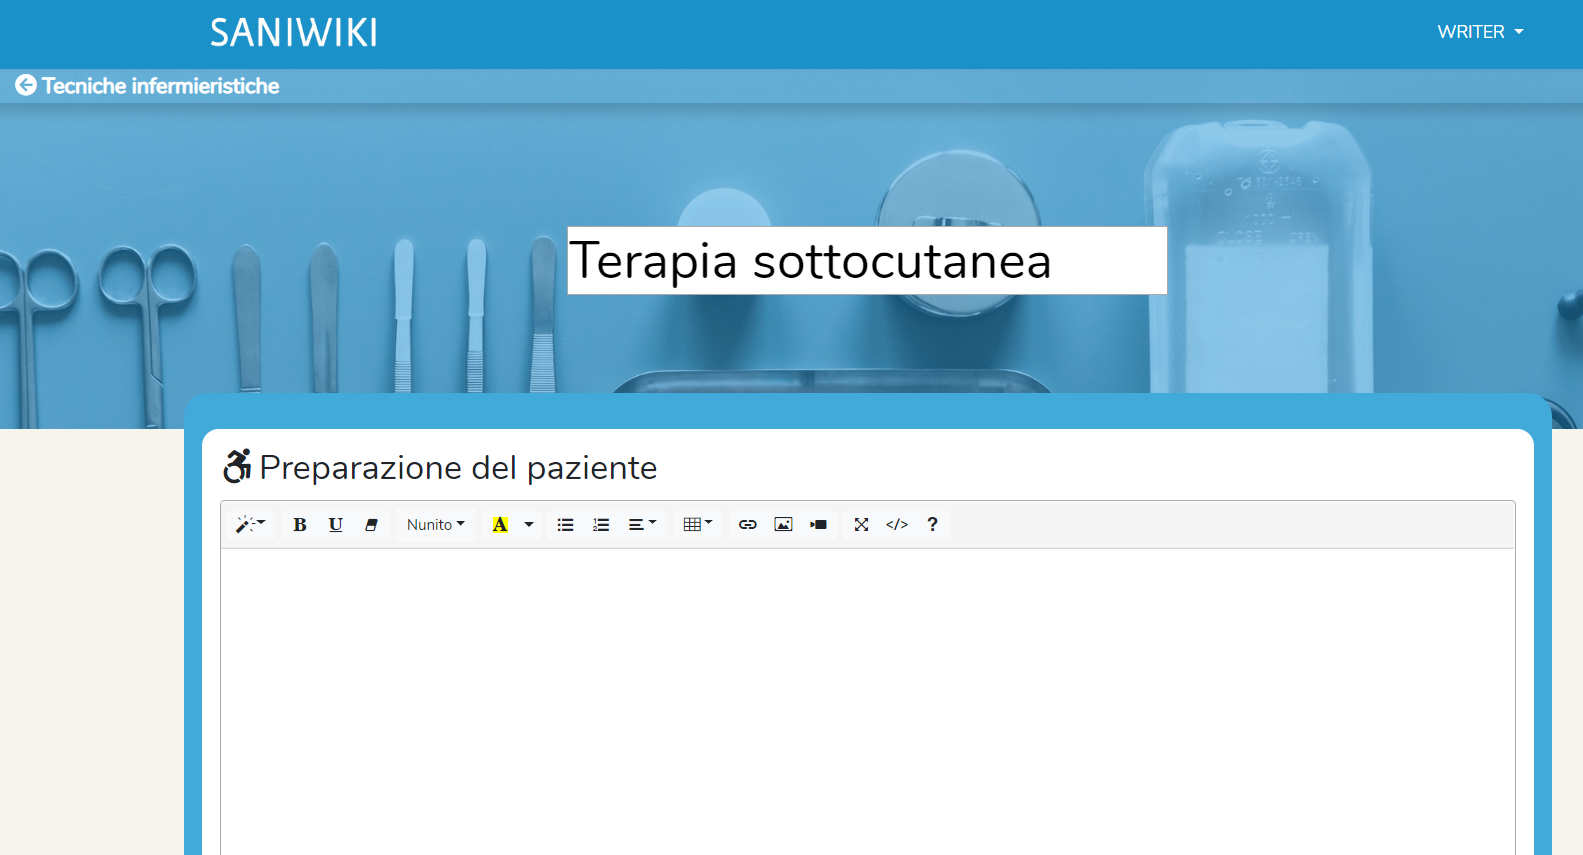
\includegraphics[scale=0.4]{saniwiki_singoloarticolo.png}
\caption{Aggiunta di un nuovo Articolo}
\end{figure}
\\\\
Accedendo alla modifica di un articolo, l'utente viene rediretto alla stessa pagina di aggiunta ma con il titolo e l'editor di testo compilati con le ultime modifiche. (Figura 4.16)\\
\begin{figure}[!h]
\centering
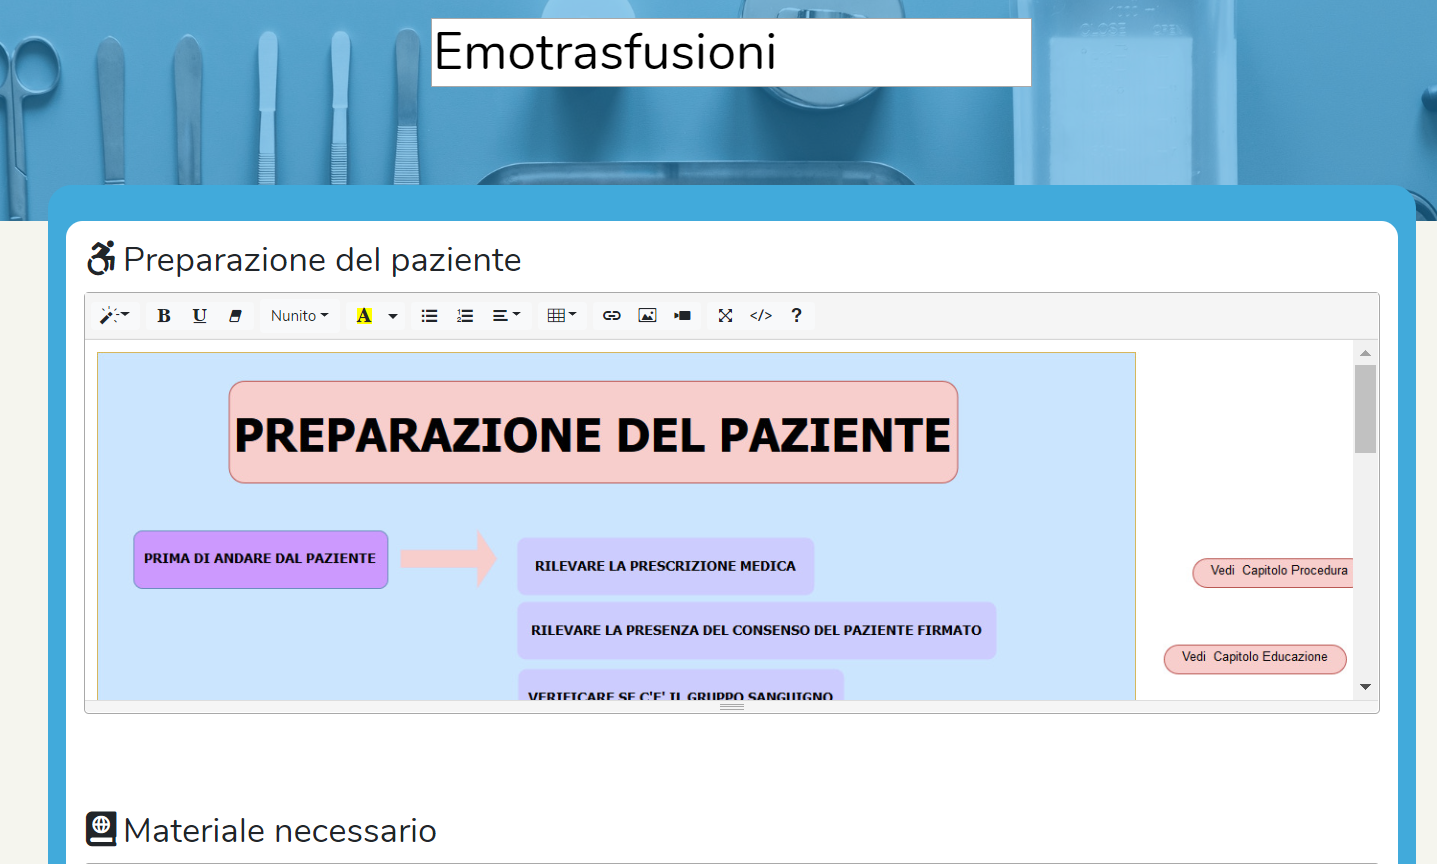
\includegraphics[scale=0.4]{saniwiki_modificaarticolo.png}
\caption{Modifica di un Articolo}
\end{figure}
\\\\
Anche per l'eliminazione di un articolo viene richiesta la conferma.

\section{Contenuti}
Per Contenuti s'intendono i vari testi presenti negli articoli, sotto alle diverse sezioni, modificabili tramite l'editor WYSYWYG. Grazie allo stesso è possibile applicare degli stili al testo e formattarlo in grassetto, sottolineato o corsivo. L'utente ha la possibilità di modificarne il font ed il colore, oltre che di allinearlo a piacimento. Altri elementi disponibili sono tabelle, links, immagini e video provenienti da una sorgente esterna. Per aggiungere questi ultimi, infatti, occorre inserirne l'URL completo.\\
L'editor a disposizione può essere mostrato anche a schermo intero per comodità, oppure ridimensionato secondo le proprie necessità durante l'inserimento dei contenuti. L'utente ha anche la possibilità di visualizzare direttamente il codice HTML generato.

\section{Barra di Ricerca}
Nella pagina principale è presente una barra di ricerca, prevista per ricercare del testo all'interno di tutti i contenuti negli articoli. La ricerca viene eseguita con una query sul database che cerca il testo immesso all'interno di tutti i contenuti. La tabella del database nella quale sono presenti tutti i contenuti è la \textit{sections\_posts}; tutti i testi vengono persistiti e ricercati nella colonna "body". I risultati di ricerca vengono successivamente presentati in un'ulteriore pagina (Figura 4.17).\\
\begin{figure}[!h]
\centering
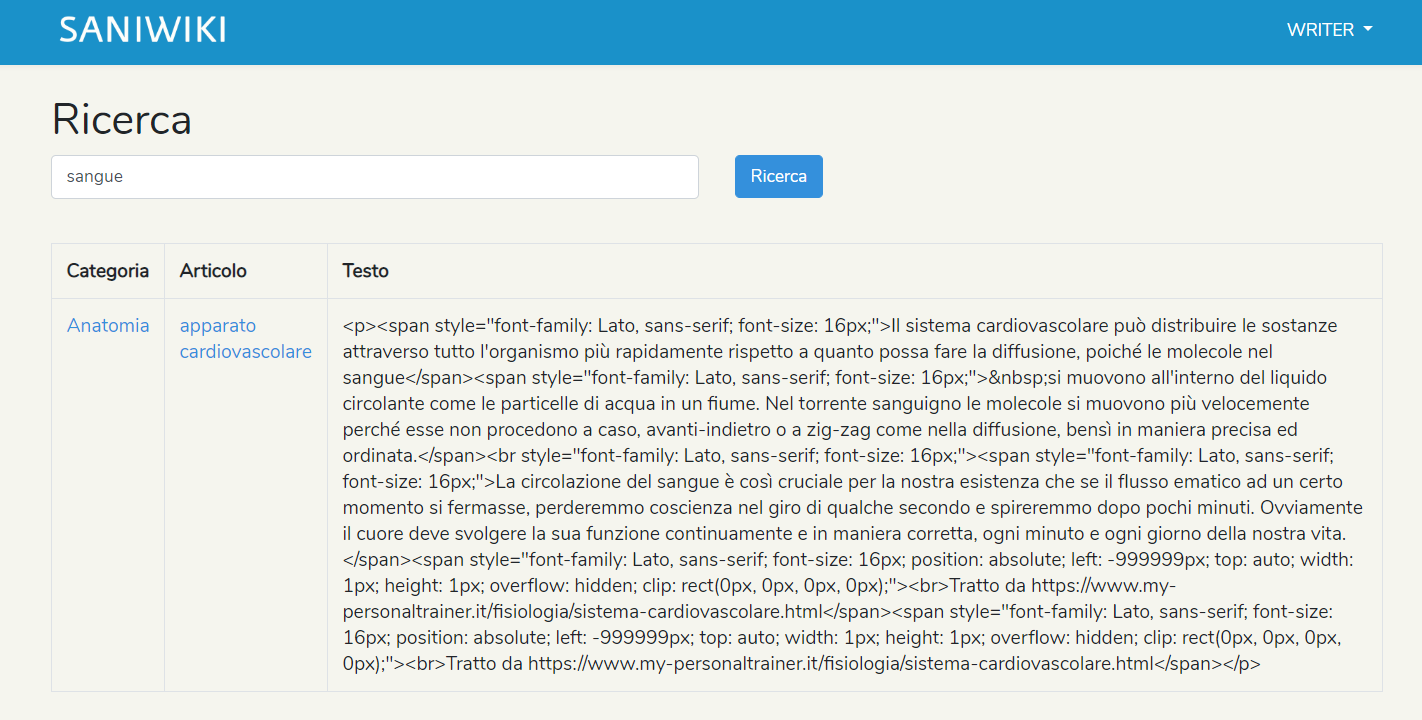
\includegraphics[scale=0.4]{saniwiki_ricerca.png}
\caption{Ricerca di contenuti}
\end{figure}
\\
Nei risultati di ricerca è possibile accedere direttamente alla pagina dell'articolo di cui fa parte un determinato testo e all'intera categoria.

\section{Icone}
Le icone che distinguono le categorie e le diverse sezioni si possono selezionare nell'aggiunta e modifica delle stesse tra una libreria di 1'480 icone messe a disposizione da Font Awesome. Tutte le immagini relative alle icone hanno un riferimento alla loro libreria esterna, pertanto non sono presenti direttamente sul server in cui è ospitata SaniWiki. Pagando un ulteriore servizio pro, con un costo di 60 dollari all'anno, sarebbe possibile ottenerne in totale 4'845 per avere una libreria più completa. Per ottenere maggiori dettagli relativi all'acquisto di un servizio pro è possibile accedere direttamente al sito della libreria esterna Font Awesome https://fontawesome.com/pro.





\chapter{Test}

\section{PHPUnit}
L'applicazione SaniWiki sviluppata in Laravel non espone delle API REST, ad eccezione di una, ovvero l'API che restituisce una lista di sezioni appartenenti ad una categoria passata come parametro: \textit{/api/sections/idCategoria}.\\
Di seguito i test effettuati nell'applicazione con PHPUnit:
\begin{verbatim}
// Get 200 status from root
    public function testGetRoot()
    {
        $response = $this->get('/');
        $response->assertStatus(200);
    }
    // Get Found status from /home
    public function testGetHome()
    {
        $response = $this->get('/home');
        $response->assertStatus(302);
    }
\end{verbatim}
Con questo test verifichiamo che accedendo alla root riceviamo un codice 200 come risposta HTTP e un codice diverso se tentiamo di accedere ad una pagina che richiede un'autorizzazione, senza averla eseguita.
\\\\
\begin{verbatim}
// Get a list of sections by a category id
    public function testGetSectionsByCategoryId() {
        $response = $this->json('GET', '/api/sections/1');
        $response->assertStatus(200);
        $response->assertJsonStructure(
            [
                [
                    'id',
                    'name',
                    'category',
                    'iconFontAw',
                    'iconURL',
                    'isIconURL',
                    'created_at',
                    'updated_at'
                ]
            ]
        );
    }
\end{verbatim}
Con questo test ci assicuriamo di ottenere una lista di una sezione per la categoria con ID "1", come attualmente corrisponde sul nostro database.

\section{Interfaccia utente}
Per garantire un buon funzionamento dell'applicazione e testarne l'usabilità per l'utente, abbiamo effettuato tutti i test di funzionamento possibili tramite interfaccia utente:
\begin{itemize}
\item Categorie: visualizzazione, inserimento, modifica, eliminazione
\item Sezioni: visualizzazione, inserimento, modifica, eliminazione
\item Articoli: visualizzazione, inserimento, modifica, eliminazione
\item Editor WYSYWYG: tutte le formattazioni di testo disponibili, inserimento di una tabella, di un link, di un'immagine e di un video, con ulteriore resize degli elementi, modifica ed eliminazione.
\item Ricerca: visualizzazione dei risultati di ricerca di parti di testo contenuti negli articoli
\item Utenti: visualizzazione, inserimento, modifica, eliminazione
\item Cambio password: cambiamento e crittografia della password immessa dall'utente
\end{itemize}





\chapter{Manuale Tecnico}

\section{Requisiti server}
Per ospitare l'applicazione SaniWiki, raccomandiamo un server con i seguenti requisiti:\\
\begin{itemize}
\item Server Linux x64\\
\item Apache HTTP Server\\
\item PHP >= v. 7.1.3\\
\item OpenSSL PHP Extension >= v. 1.0.1\\
\item PDO PHP Extension >= 7.1.3\\
\item Mbstring PHP Extension >= 7.1.3\\
\item Tokenizer PHP Extension >= 7.1.3\\
\item XML PHP Extension >= 7.1.3\\
\item Ctype PHP Extension >= 7.1.3\\
\item JSON PHP Extension >= 7.1.3\\
\item BCMath PHP Extension >= 7.1.3\\
\item Database MySQL >= v. 5.6 o MariaDB >= v. 10.0\\
\item Composer >= v. 1.7.3
\end{itemize}
\begin{figure}[!h]
\centering

\includegraphics[scale=0.7]{requirements.png}
\caption{Requisiti}
\end{figure}

\section{Configurazioni server}
Nel caso di un server CentOS con SELinux abilitato, questo potrebbe dare dei problemi sul funzionamento dell'applicazione; è consigliato pertanto disabilitare SELinux.\\
Un'altra configurazione da applicare riguarda i permessi alla cartella /storage, in quanto la stessa cartella contiene i log di Laravel e il sistema deve avere il permesso di scrivere negli stessi files:
\begin{verbatim}
sudo chmod -R 777 /storage
\end{verbatim}
Nella configurazione del virtualhost di Apache, è importante che a livello della directory principale sia specificato AllowOverrideAll:
\begin{verbatim}
<Directory /directoryPrincipale>
	Options FollowSymLinks MultiViews
	AllowOverride All
	Order allow,deny
	allow from all
	Require all granted
</Directory>
\end{verbatim}

\section{Nuova installazione su server}
Per installare una nuova applicazione di SaniWiki su un server, è possibile procedere in due modi: tramite la copia dei files direttamente sul server oppure la copia tramite Git. Entrambe le procedure sono descritte di seguito.

\subsection{Copia}
Dopo aver configurato il virtualhost di Apache dedicato a SaniWiki, occorre copiare tutti i files relativi all'applicazione nella directory principale (home directory configurata in Apache). Assicurarsi di configurare i permessi corretti alla cartella /storage, come descritto precedentemente. L'applicazione necessita di un database MySQL dedicato; i dati relativi al nome del database, nome utente e password vanno configurati nel file .env presente nella directory principale.\\
\begin{itemize}
\item Per creare tutte le tabelle in banca dati, nella directory principale lanciare il comando:
\begin{verbatim}
php artisan migrate:fresh
\end{verbatim}
\item Per creare tutte le tabelle in banca dati e riempire la tabella "users" con tre utenti di test (Admin, Writer, Reader), nella directory principale lanciare il comando:
\begin{verbatim}
php artisan migrate:fresh --seed
\end{verbatim}
\end{itemize}

\subsection{Git Clone}
Per installare una nuova copia di SaniWiki tramite git, eseguire un git clone nella cartella principale desiderata. Creare un nuovo database MySQL e configurare i dati relativi al nome del database, nome utente e password nel file .env presente nella directory principale. Procedere con l'esecuzione dei seguenti comandi, posizionandosi nella cartella principale:
\begin{itemize}
\item \begin{verbatim}composer install\end{verbatim}
\item \begin{verbatim}php artisan key:generate\end{verbatim}
\item Per creare tutte le tabelle in banca dati, nella directory principale lanciare il comando:
\begin{verbatim}
php artisan migrate:fresh
\end{verbatim}
\item Per creare tutte le tabelle in banca dati e riempire la tabella "users" con tre utenti di test (Admin, Writer, Reader), nella directory principale lanciare il comando:
\begin{verbatim}
php artisan migrate:fresh --seed
\end{verbatim}
\end{itemize}

\section{Comandi utili e risoluzioni}
\begin{itemize}
\item Nel caso in cui il comando \textit{php artisan migrate:fresh --seed} dovesse dare problemi nell'inserimento dei dati nel database, eseguire:
\begin{verbatim}
composer dump-autoload
\end{verbatim}
Questo comando rigenera la lista delle classi necessarie da includere nel progetto e corregge dei problemi che si creano quando vengono definite nuove classi.
\item Per qualsiasi altro problema che si presenta in Laravel, prima di eseguire una ricerca sull'errore provare a lanciare i comandi seguenti:
\begin{verbatim}
composer dump-autoload
composer install
\end{verbatim}
\end{itemize}

\section{Configurazione client raccomandata per dispositivi mobili Android}
Siccome l'applicazione SaniWiki è responsive e adattata per dispositivi mobili, raccomandiamo la seguente installazione sui dispositivi mobili Android. Questa configurazione permette di utilizzare la piattaforma in modo più agevole.
\begin{itemize}
\item Aprire il browser e accedere all'indirizzo principale di SaniWiki
\item Selezionare l'icona delle impostazioni (tre puntini) in alto a destra (Figura 6.2)
\item Selezionare "Aggiungi a schermata Home" (Figura 6.3)
\item Uscire dal browser, nella propria schermata Home sarà presente l'icona SaniWiki (Figura 6.4)
\item Utilizzare SaniWiki aprendo l'icona della schermata Home
\end{itemize}
\begin{figure}[!h]
\centering
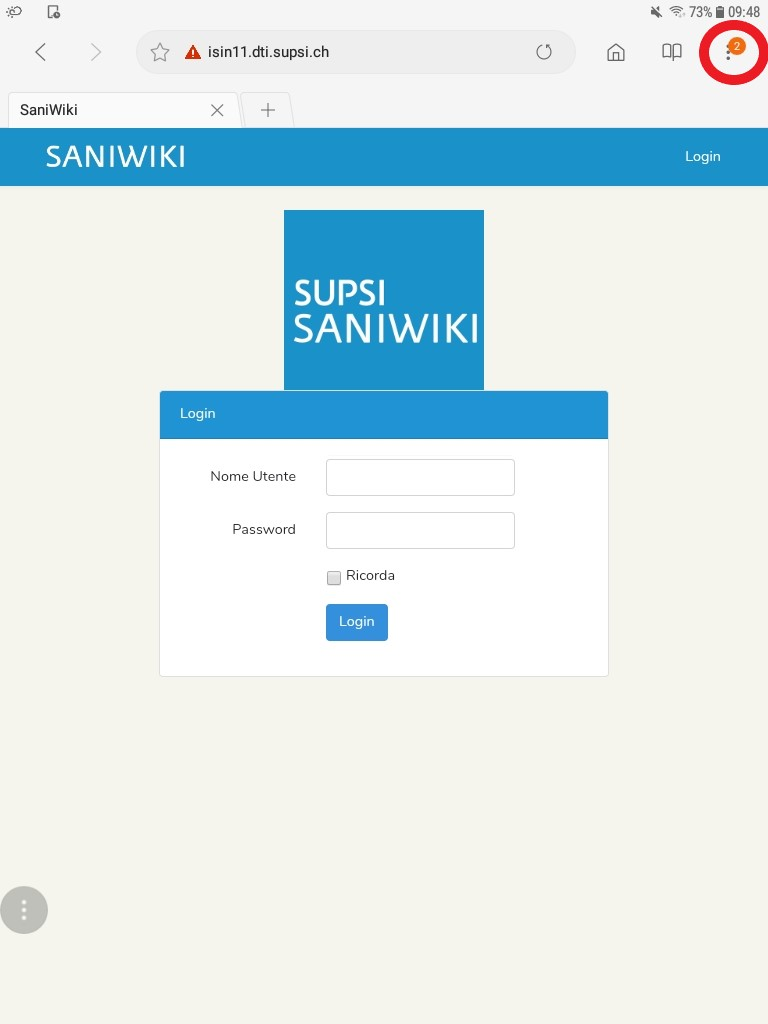
\includegraphics[scale=0.3]{saniwiki_android1.png}
\caption{Android - Impostazioni del browser}
\end{figure}
\begin{figure}[!h]
\centering
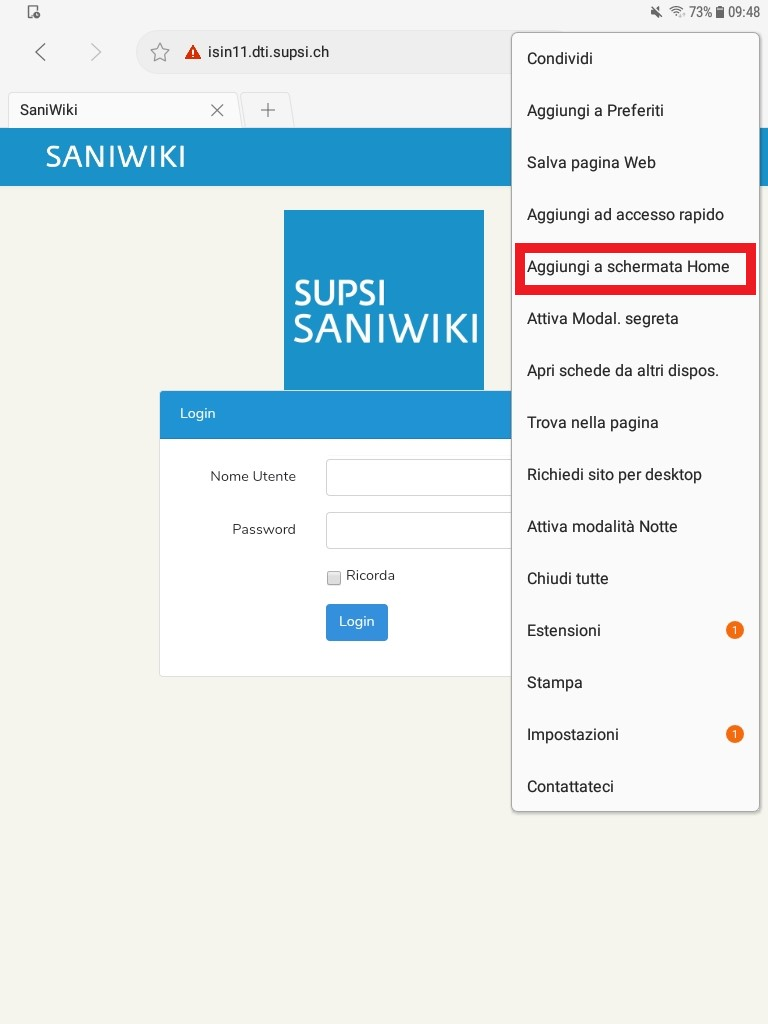
\includegraphics[scale=0.3]{saniwiki_android2.png}
\caption{Android - Aggiunta alla schermata Home}
\end{figure}
\begin{figure}[!h]
\centering

\includegraphics[scale=0.4]{saniwiki_android3.png}
\caption{Android - Icona SaniWiki}
\end{figure}




\chapter{Conclusioni}

\section{Problemi riscontrati}
\begin{itemize}
\item \textbf{Scelta del framework}: non avendo nessuna esperienza nel campo delle applicazioni web, il primo problema affrontato è stato quello della ricerca, valutazione e scelta del framework da utilizzare. Il primo modulo di Applicazioni web è iniziato parallelamente al progetto SaniWiki e non avevamo le totali competenze per sviluppare un'applicazione di questo livello di complessità, considerando tutti i requisiti richiesti dai committenti. Giunti a fine progetto e a fine modulo di Applicazioni web, probabilmente se dovessimo affrontare nuovamente delle considerazioni simili prenderemmo in considerazione anche altri framework, come Java Spring, che abbiamo avuto la possibilità di approfondire molto durante le lezioni di questo semestre.\\
La scelta del framework è stata uno dei fattori che ci ha fatto perdere diverso tempo, non solo per quanto riguarda la ricerca, ma anche per una prima implementazione di SaniWiki utilizzando Lumen, il microframework di Laravel, che abbiamo deciso in un secondo momento di scartare in quanto questo non offre diverse funzionalità, al contrario di Laravel, che alla fine ci hanno reso il lavoro meno ostacolato e più funzionale.
\item \textbf{Scarso supporto}: i primi approcci con Lumen e Laravel sono stati parecchio difficoltosi a causa della nostra mancata esperienza con le applicazioni web. Abbiamo dunque cercato supporto presso alcuni docenti che lavorano nel campo ma alcuni tentativi si sono rivelati superflui, in quanto quasi nessuno conosce questi due framework sui quali ci siamo concentrati. Malgrado ciò, siamo riusciti ad ottenere degli ottimi consigli sulle applicazioni responsive, javascript e altri piccoli particolari che hanno fatto la differenza.
\item \textbf{Bisogni non totalmente definiti dai committenti}: inizialmente vi era un po' di confusione su quelli che erano realmente i bisogni dei committenti. In modo particolare, la struttura che avrebbe dovuto assumere l'applicazione per organizzare le informazioni risultava poco chiara. Dopo un paio di incontri siamo riusciti a chiarire meglio le loro necessità e a studiare una soluzione insieme. Per noi sarebbe stato significativo ricevere degli esempi di testi e immagini basati sulla soluzione discussa come richiesto a loro, documentazione che non abbiamo mai ricevuto nel corso degli ultimi mesi. Per questo motivo abbiamo poi preso posizione nel decidere definitivamente la struttura con categorie e sezioni imposte come template per la definizione dei diversi articoli.
\item \textbf{Icone scartate}: in un primo mockup mostrato alle committenti erano state definite le diverse categorie con delle icone che gli utenti avrebbero potuto caricare e utilizzare nel sistema. Discutendo con loro, però, è sorto un problema di trattamento immagini e il lavoro di ricerca e caricamento icone non sarebbe stato così semplice per loro. Per questo motivo abbiamo deciso di sfruttare la libreria esterna di FontAwesome, che rende molto più facile la selezione delle icone per le categorie e le sezioni.
\item \textbf{Immagine di sfondo diversa per ogni categoria, non implementato}: nell'ultimo incontro con le committenti ci è stato richiesto di poter modificare l'immagine di sfondo a seconda della categoria selezionata. Per motivi tempistici e di complessità, non siamo riusciti a sviluppare una parte di caricamento delle immagini e visualizzazione in tempi previsti per la consegna del progetto.
\item \textbf{Modali di Bootstrap}: per rendere l'interfaccia utente più dinamica e piacevole da utilizzare, abbiamo sfruttato i modali di Bootstrap, che non si sono rivelati semplici da gestire. In modo particolare per quanto riguarda la modifica delle categorie, sezioni, articoli ed utenti, in quanto avrebbe richiesto delle competenze di base di javascript, non in nostro possesso. Questo problema ci ha fatto perdere diverso tempo per la ricerca delle soluzioni possibili e lo sviluppo di test necessari.
\item \textbf{Versioni di Laravel e Bootstrap}: lo sviluppo di alcune funzionalità, utilizzando le nuove versioni utilizzate di Laravel (5.7) e Bootstrap (4.0), è risultato abbastanza difficoltoso.
\item \textbf{Versione di Ionic}: nella fase iniziale di ricerca del framework, avevamo valutato l'utilizzo di Ionic integrato con Laravel. Lo sviluppo con lo stesso non è stato possibile in quanto la versione recente utilizzata di Ionic non rendeva possibile l'integrazione con Laravel e/o Lumen.
\end{itemize}

\section{Sviluppi futuri}
SaniWiki ha un'ottima base di partenza, concepita per essere espansa e per migliorare l'efficacia di comunicazione verso i suoi utenti. Uno dei punti più interessanti è sicuramente la possibilità di interfacciarsi al framework di Laravel con Ionic, implementando così una Web App nativa e fornendo a sua volta un supporto più veloce, ottimizzato e adatto ad ogni dispositivo iOS e Android.\\
Si potrebbe implementare, in fase di creazione, l'aggiunta di uno sfondo per ogni singola categoria. Questa funzionalità è stata già inizialmente concepita a livello di struttura del database, ma non completamente implementata. Grazie ad una colonna con il nome "bgImage" nella tabella "categories", dove attualmente viene salvato al suo interno il percorso di un'immagine di default attraverso il controller specifico, sarà sufficiente modificare in fase di creazione della categoria, l'immagine sul server e salvare l'indirizzo specifico sulla tabella.  Per quanto riguarda la visualizzazione nel template di Blade, la view è già stata finalizzata per leggere lo sfondo da quella tabella.\\
Concludendo, SaniWiki, come ogni piattaforma, avrà bisogno comunque di manutenzione e di test da parte degli utenti per conoscere le necessità didattiche effettive di cui ha realmente bisogno. Solo dopo aver raccolto osservazioni e critiche da parte degli utilizzatori si potrà effettuare un'ulteriore analisi per valutare l'offerta di possibili sviluppi futuri.\\
Per quanto riguarda la sicurezza, una volta che SaniWiki verrà messa in produzione, raccomandiamo l'installazione e la configurazione di un certificato di sicurezza per accedere alla piattaforma tramite il protocollo HTTPS anziché HTTP.




\chapter{Piani di lavoro}
Nei requisiti iniziali del relatore, era stato richiesto l'utilizzo di SCRUM (SCM) per lo sviluppo dell'applicazione. Abbiamo avuto la possibilità di organizzare la pianificazione del lavoro in diversi Sprint. Di seguito riportiamo lo Sprint board e lo Sprint burndown dello Sprint 7, il quale è iniziato il 09.12.2018 ed è finito il 15.12.2018 (Figura 8.1 e 8.2).\\
\begin{figure}[!h]
\centering
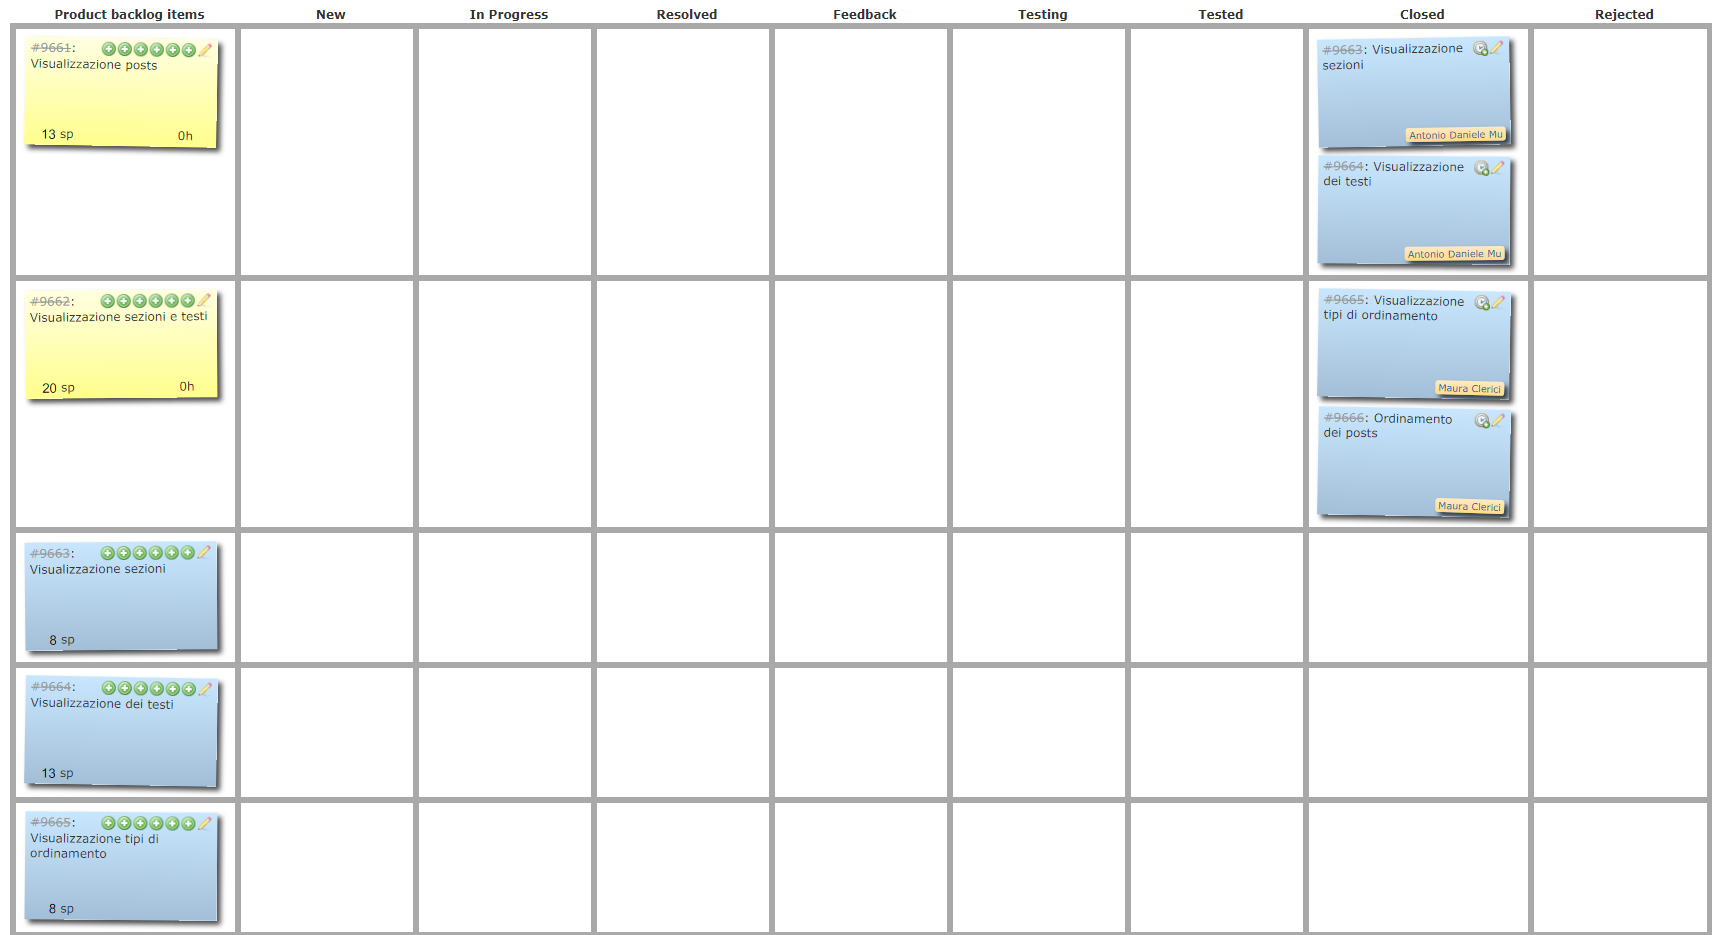
\includegraphics[scale=0.35]{sprint7board.png}
\caption{Sprint7 - Sprint Board}
\end{figure}
\begin{figure}[!h]
\centering
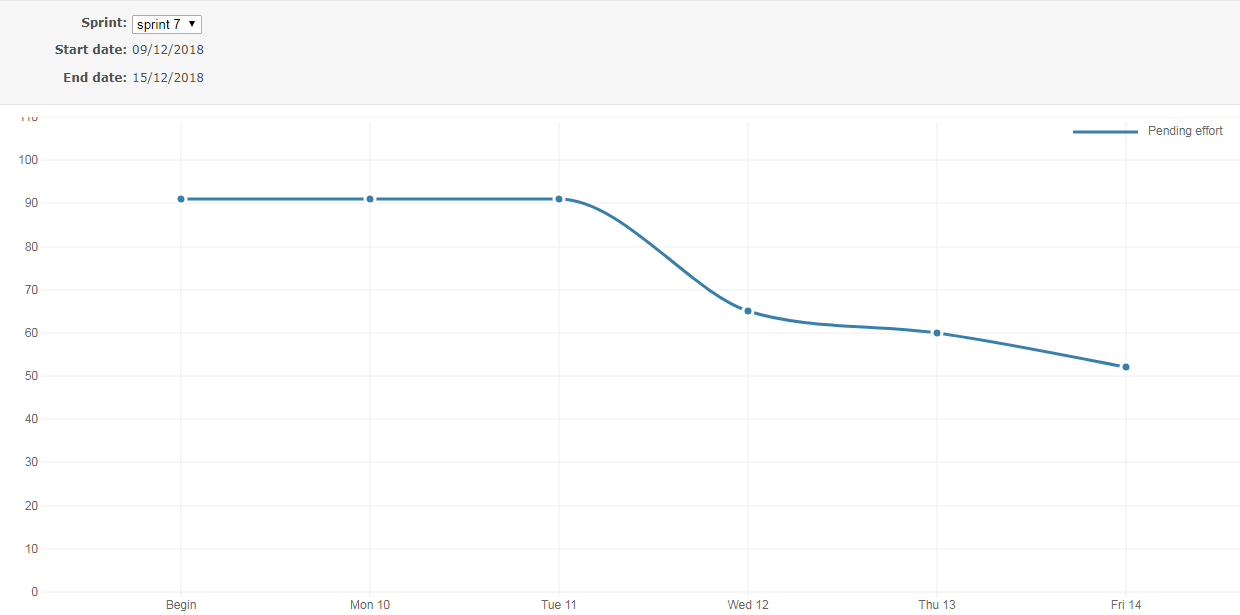
\includegraphics[scale=0.3]{sprint7.png}
\caption{Sprint7 - Sprint Burndown}
\end{figure}
\\\\\\\\\\\\\\\\
Lo Sprint riportato rappresenta una fase importante per lo sviluppo del progetto, in quanto durante quel periodo sono state implementate alcune delle funzionalità di visualizzazione più importanti.\\
Osservando i diversi Sprint, a lavoro terminato, abbiamo avuto la possibilità di valutare la fase iniziale di ricerca e scelta dei framework: da inizio ottobre fino al 9 novembre 2018 è stato testato Lumen e Ionic e non vi è stato un vero e proprio sviluppo di SaniWiki. Dal 9 novembre 2018 in avanti è stata installata la versione definitiva di Laravel, sulla quale sono state sviluppate tutte le funzionalità del progetto. Analizzando in modo più approfondito l'andamento e il tempo impiegato, possiamo considerare quanto tempo è servito per sviluppare le prime funzionalità semplici e come questo tempo sia diminuito man mano che acquisivamo esperienza nella materia.





\chapter{Fonti}
\begin{itemize}
\item Laravel Tutorial: Step by Step Guide to Building Your First Laravel Application\\
https://laravel-news.com/your-first-laravel-application
\item Generating fake Seeds data with Faker package\\
https://laraveldaily.com/generating-fake-seeds-data-with-faker-package
\item Laravel 5.7 From Scratch\\
https://laracasts.com/series/laravel-from-scratch-2018
\item Bootstrap 4.0 Modal\\
https://getbootstrap.com/docs/4.0/components/modal
\item Lumen Docs\\
https://lumen.laravel.com/docs/5.7
\item Laravel Docs\\
https://laravel.com/docs/5.7/installation
\item Troubleshooting\\
https://stackoverflow.com
\end{itemize}





\chapter{Allegati}
\begin{itemize}
\item Schema del database esteso
\item Mockup di SaniWiki iniziale
\item Dati di accesso alla piattaforma di test
\item Diagrammi dei casi d'uso
\end{itemize}


\newpage
\end{document}
